\documentclass[conference,onecolumn]{IEEEtran}
\IEEEoverridecommandlockouts
% The preceding line is only needed to identify funding in the first footnote. If that is unneeded, please comment it out.
\usepackage{cite}
\usepackage{amsmath,amssymb,amsfonts}
\usepackage{algorithmic}
\usepackage{graphicx}
\usepackage{subfig}
\graphicspath{{./Figures/}}
\usepackage{textcomp}
\usepackage{xcolor}
\usepackage{listings}
\usepackage{bm}
\def\BibTeX{{\rm B\kern-.05em{\sc i\kern-.025em b}\kern-.08em
    T\kern-.1667em\lower.7ex\hbox{E}\kern-.125emX}}

\lstset{
	backgroundcolor=\color{lightgray},
	rulesepcolor= \color{gray}, 
	breaklines=true,  
	numbers=left, 
	numberstyle= \small,
	keywordstyle= \color{blue}, 
	commentstyle=\color{green!50!black},
	captionpos=b,
	language=R
}


\begin{document}

\title{Report}
\author{\IEEEauthorblockN{Zhang Weini}
\IEEEauthorblockA{Student Number: 23020181154257}}

\maketitle

%\begin{abstract}
%This document is a model and instructions for \LaTeX.
%This and the IEEEtran.cls file define the components of your paper [title, text, heads, etc.]. *CRITICAL: Do Not Use Symbols, Special Characters, Footnotes, 
%or Math in Paper Title or Abstract.
%\end{abstract}

%\begin{IEEEkeywords}
%component, formatting, style, styling, insert
%\end{IEEEkeywords}

\section{Assignment 1 (2019-07-15)}
\subsection{Read, summarize and comment the article}

\textbf{* Relevance}
	
The main purpose of this paper is to test the computational accuracy of some numerical scientific platforms, under the diversity of operational systems.

Assessing the accuracy of these platforms is important. In many fields, to find best approximate solutions to the problem, we have high requirements on computational accuracy. Especially when solving complex models with many variables and values, minute errors in each step may have great effect on the final results. 

The authors think previous studies were limited to simply comparing results with certified values provided by Statistical Reference Datasets. Thus, based on this method, they design their experiments to test the accuracy of these platforms.
	
\textbf{* Methodology}
	
To assess the accuracy of \textit{Octave 3.2.4}, \textit{Scilab 5.3} and \textit{Matlab R2011a} platforms, under three operating systems (\textit{Windows}, \textit{Ubuntu} and \textit{Mac OS}) and the hardware(\textit{i386 architecture}), the authors conduct two groups of experiments, in which they compare the results computed by the platforms with certified values:
\begin{itemize}
	\item \textit{Statistical description tests (certified values provided by NIST)}
	\begin{enumerate}
		\item Basic statistics
		\subitem Assessment: (1)mean, (2)standard deviation (3)first lag coefficient of autocorrelation
		\subitem Measurement: LRE + the bootstrap estimates of the standard deviation of LREs
		\subitem Using Monte Carlo study
		
		\item Probability distribution functions
		\subitem Assessment: (1)binomial, (2)Poisson, (3)gamma, (4)normal, (5)$\chi^2$, (6)beta, (7)t-Student, (8)F
		\subitem Measurement: LRE
		
		\item Linear regression
		\subitem Measurement: the smallest LRE + the LRE of RSD
	\end{enumerate}
				
	\item \textit{Matrices operations tests}
	\begin{enumerate}
		\item Determinant computation
		\subitem Assessment: Compute the determinant of ill-conditioned $2\times 2$ matrices.
		\subitem Measurement: Logical comparesion of computed value and certified value 0.
		
		\item Spectral graph analysis
		\subitem Compute the eigenvalues of the Laplacian matrix of a bipartite graph.
		\subitem Measurement: LREs and percentage of some values associated with eigenvalues
	\end{enumerate}	
\end{itemize}

\textbf{* Results and conclusions}

In this paper, the authors show the results of their experiments in several tables. From the results they have the following conclusion:
\begin{enumerate}
	\item Basic statistics
	\begin{itemize}
		\item \textit{Mean}: Octave for Linux presents relatively low accuracy, other platforms perform well on the datasets.
		\item \textit{Standard deviation}: Octave presents the best results while Scilab presents an unacceptable low accuracy in a single dataset.
		\item \textit{First-lag sample autocorrelation}: none of the platforms provides acceptable results. Scilab has the worst performance.
		\item \textit{Stability}: Scilab is the worst platform. Octave for Linux is also instable when computing the sample mean and the sample standard deviation.
	\end{itemize}
	
	\item Probability distribution functions
	\begin{itemize}
		\item \textit{Binomial and t-Student distributions}: Scilab presents the best performance. Octave provides unacceptable results. Matlab and Octave fails at computing the t-Student distribution.
		\item \textit{Poisson law}: Scilab presents the best performance when computing the cumulative distribution function.
		\item \textit{Gamma law}: All the three platforms are acceptable.
		\item \textit{F distribution}: Octave presents the best performance.
		\item \textit{Normal distribution}: MatLab and Octave provides the same good results, while Scilab provides bad results.
	\end{itemize}

	\item Linear regression
	\begin{itemize}
		\item No single platform is credible for the linear regression problems.
	\end{itemize}

	\item Determinant computation
	\begin{itemize}
		\item All the three platforms provide the same acceptable results.
	\end{itemize}

	\item Spectral graph analysis
	\begin{itemize}
		\item The bigger the graph, the worse the results.
		\item Double-precision computation is recommended. When comparing to known values, use floating point representation at most.
		\item Variability: MatLab and Octave are equivalent and more consistent than Scilab. 
	\end{itemize}

\end{enumerate}

\textbf{* Comments}

First, the main highlights of this paper include: (1) Using Monte Carlo studies to assess the stability of the results with respect to small departures from the original input. (2) Besides statistical description tests, the authors assess a set of matrix operations.

Second, I doubt whether the experiments in this paper can objectively evaluate the accuracy of the platforms. The datasets used in the experiments are limited. I'm not sure if the performance of these platforms is consistent with the conclusions of this paper when using other datasets.

Third, as mentioned in this paper, their results are not consistent with some previous work. I wonder what causes the inconsistency of the results. Is it because the experimental scheme has some problems or the platforms are instable? If the instability of these platforms affects the experimental results, are the results in this paper credible?

Finally, this paper can provide a reference for me when I need to choose a high precision and stable numerical scientific platform to solve problems.


\section{Assignment 2 (2019-07-16)}
\subsection{Exercise 4.4: Obtain the expression of the density of $\mathcal K$-distributed amplitude data via the transformation $Z_A=\sqrt{Z_I}$. Compute its moments. Illustrate.}

For $Z_I \sim \mathcal K(\alpha,\lambda,L)$, the density of $Z_I$ is:
\begin{equation}
f_{Z_I}(z_I;\alpha,\lambda,L)=\frac{2\lambda L}{\Gamma(\alpha)\Gamma(L)} (\lambda L z_I)^{\frac{\alpha+L}{2}-1} k_{\alpha-L}(2\sqrt{\lambda L z_I})
\label{eq:ZI_K_dis}
\end{equation}

The density of amplitude data $Z_A = g(Z_I)=\sqrt{Z_I}$ is given by:
\begin{equation}
\begin{split}
f_{Z_A}(z_A;\alpha,\lambda,L) &= \frac{2\lambda L}{\Gamma(\alpha)\Gamma(L)} (g^{-1}(z_A))^{'} (\lambda L g^{-1}(z_A))^{\frac{\alpha+L}{2}-1} k_{\alpha-L}(2\sqrt{\lambda L g^{-1}(z_A)})  \\
&= \frac{2\lambda L}{\Gamma(\alpha)\Gamma(L)} 2z_A (\lambda L z_A^2)^{\frac{\alpha+L}{2}-1} k_{\alpha-L}(2\sqrt{\lambda L z_A^2}) \\
&=  \frac{4\lambda L}{\Gamma(\alpha)\Gamma(L)} (\lambda L)^{\frac{\alpha+L}{2}-1} z_A^{\alpha+L-1} k_{\alpha-L}(2\sqrt{\lambda L z_A^2})
\end{split}
\label{eq:ZA_K_dis}
\end{equation}

The k-order moments of $Z_A$ are:
\begin{equation}
\begin{split}
E(Z_A^k) &= E(Z_I^{\frac{k}{2}}) \\
&= (\lambda L)^{-\frac{k}{2}} \frac{\Gamma(L+\frac{k}{2})\Gamma(\alpha+\frac{k}{2})}{\Gamma(L)\Gamma(\alpha)}
\end{split}
\label{eq:Moment_ZA_k_dis}
\end{equation}


\subsection{Exercise 4.8: Obtain the expression of the density of $\mathcal G^0$-distributed amplitude data via the transformation $Z_A=\sqrt{Z_I}$. Compute its moments. Illustrate.} 

For $Z_I \sim \mathcal G^0(\alpha,\gamma,L)$, the density of $Z_I$ is:
\begin{equation}
f_{Z_I}(z_I;\alpha,\gamma,L) = \frac{L^L \Gamma(L-\alpha)}{\gamma^\alpha \Gamma(L)\Gamma(-\alpha)} \frac{z_I^{L-1}}{(\gamma+L z_I)^{L-\alpha}}
\label{eq:ZI_G0_dis}
\end{equation}

The density of amplitude data $Z_A = g(Z_I)=\sqrt{Z_I}$ is given by:
\begin{equation}
\begin{split}
f_{Z_A}(z_A;\alpha,\gamma,L) &= \frac{L^L \Gamma(L-\alpha)}{\gamma^\alpha \Gamma(L)\Gamma(-\alpha)} (g^{-1}(z_A))^{'} \frac{(g^{-1}(z_A))^{L-1}}{(\gamma+L g^{-1}(z_A))^{L-\alpha}} \\
&= \frac{L^L \Gamma(L-\alpha)}{\gamma^\alpha \Gamma(L)\Gamma(-\alpha)} 2z_A \frac{(z_A^2)^{L-1}}{(\gamma+L z_A^2)^{L-\alpha}} \\
&= \frac{2L^L \Gamma(L-\alpha)}{\gamma^\alpha \Gamma(L)\Gamma(-\alpha)} \frac{z_A^{2L-1}}{(\gamma+L z_A^2)^{L-\alpha}}
\end{split}
\label{eq:ZA_G0_dis}
\end{equation}

The k-order moments of $Z_A$ are:
\begin{equation}
\begin{split}
E(Z_A^k) &= E(Z_I^{\frac{k}{2}}) \\
&= (\gamma / L)^{\frac{k}{2}} \frac{\Gamma(L+\frac{k}{2})\Gamma(-\alpha-\frac{k}{2})}{\Gamma(L)\Gamma(-\alpha)}
\end{split}
\label{eq:Moment_ZA_G0_dis}
\end{equation}


\subsection{Assign Beta histograms to the channels of both the dark and bright image to obtain different visualizations.}

First, I equalize each channel of \textit{dark} and \textit{bright} data, and also assign Beta histograms to each channel. Fig.\ref{Fig:LiEqBe_dark} is the visualization of \textit{dark} data. Fig.\ref{Fig:LiEqBe_dark}\subref{Fig:Linearized_dark}, \ref{Fig:LiEqBe_dark}\subref{Fig:Equalized_dark} and \ref{Fig:LiEqBe_dark}\subref{Fig:BetaHistograms_dark} show the linearization, equalization and $\mathcal{B}(8,8)$ stipulation of \textit{dark} data, respectively. Because the data contains a very broad range and most of the values are clustered in low interval(shown in Fig.\ref{Fig:hist_dark_LiEqBe}), little is visible in Fig.\ref{Fig:LiEqBe_dark}\subref{Fig:Linearized_dark}, and Fig. \ref{Fig:LiEqBe_dark}\subref{Fig:Equalized_dark} looks exaggerated. Compared with linearized data and equalized data, the data with $\mathcal{B}(8,8)$ histograms is more visible and less exaggerated.  
\begin{figure}[htbp]
	\centering
	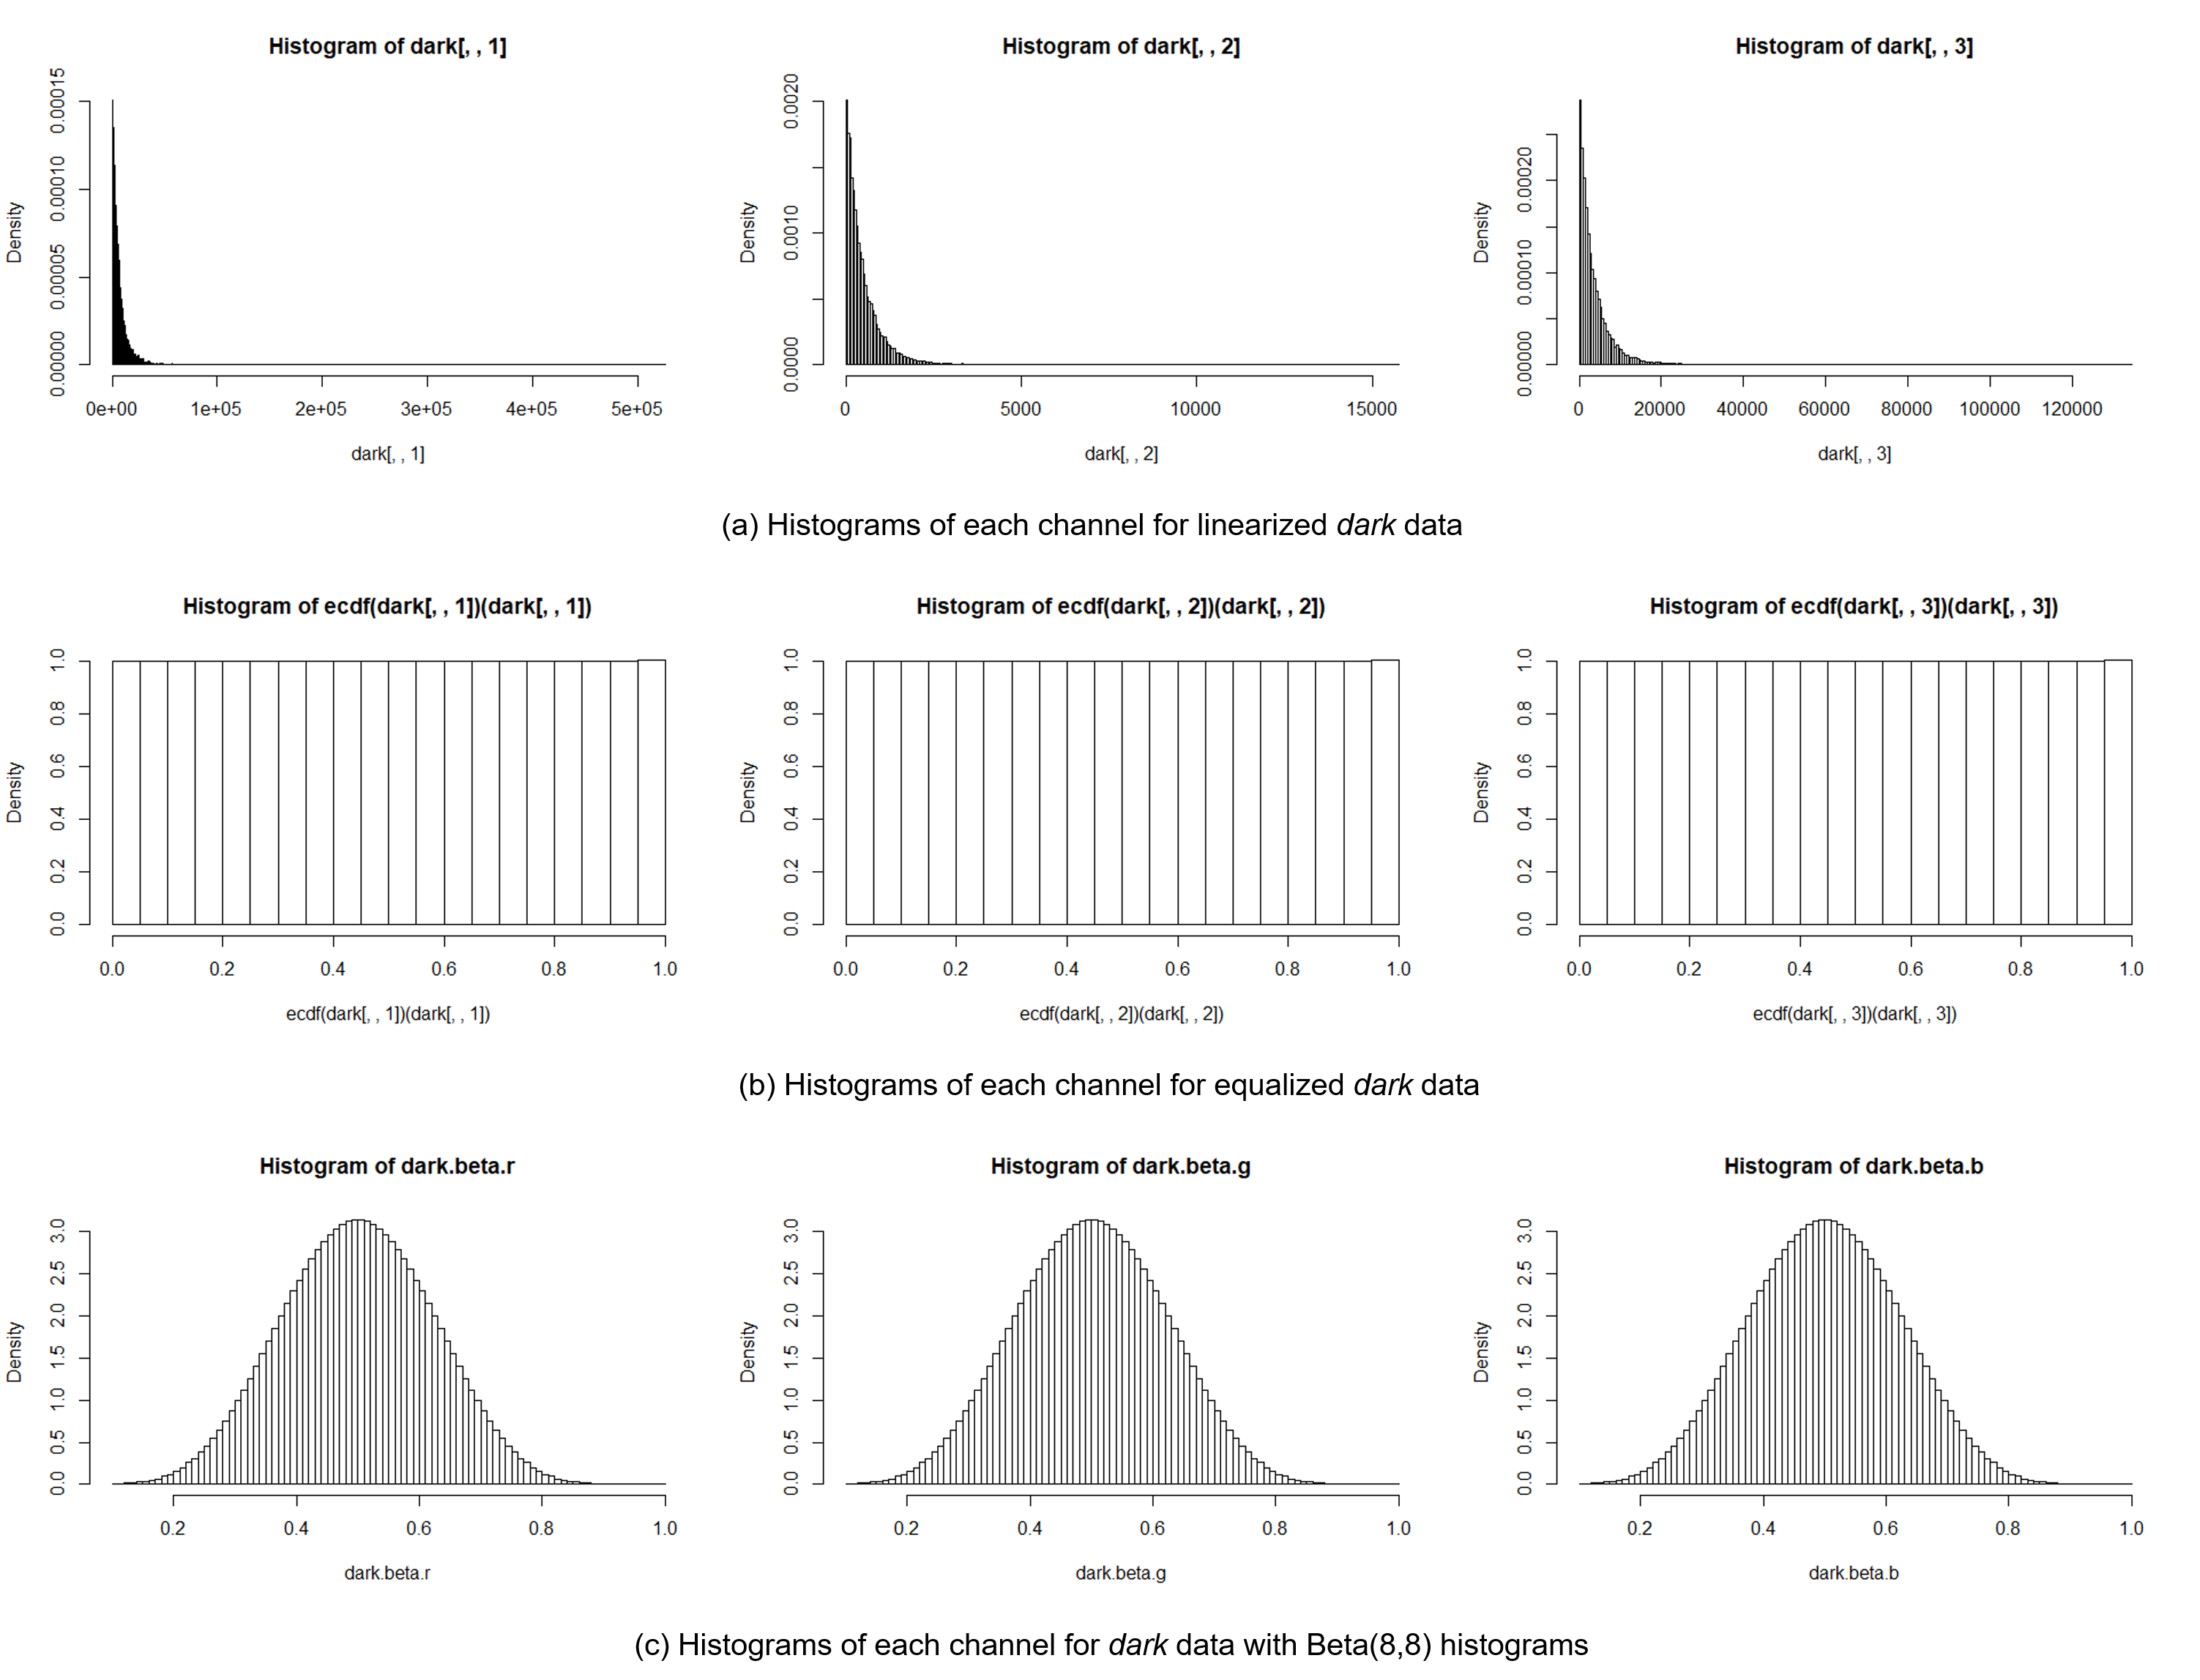
\includegraphics[width=.8\linewidth]{hist_dark_LiEqBe.png}
	\caption{Histograms of each channel for Linearized, equalized and $\mathcal{B}(8,8)$ stipulated \textit{dark} data}
	\label{Fig:hist_dark_LiEqBe}
\end{figure}

\begin{figure*}[htb]
	\centering
	\subfloat[Linearized \textit{dark} data\label{Fig:Linearized_dark}]{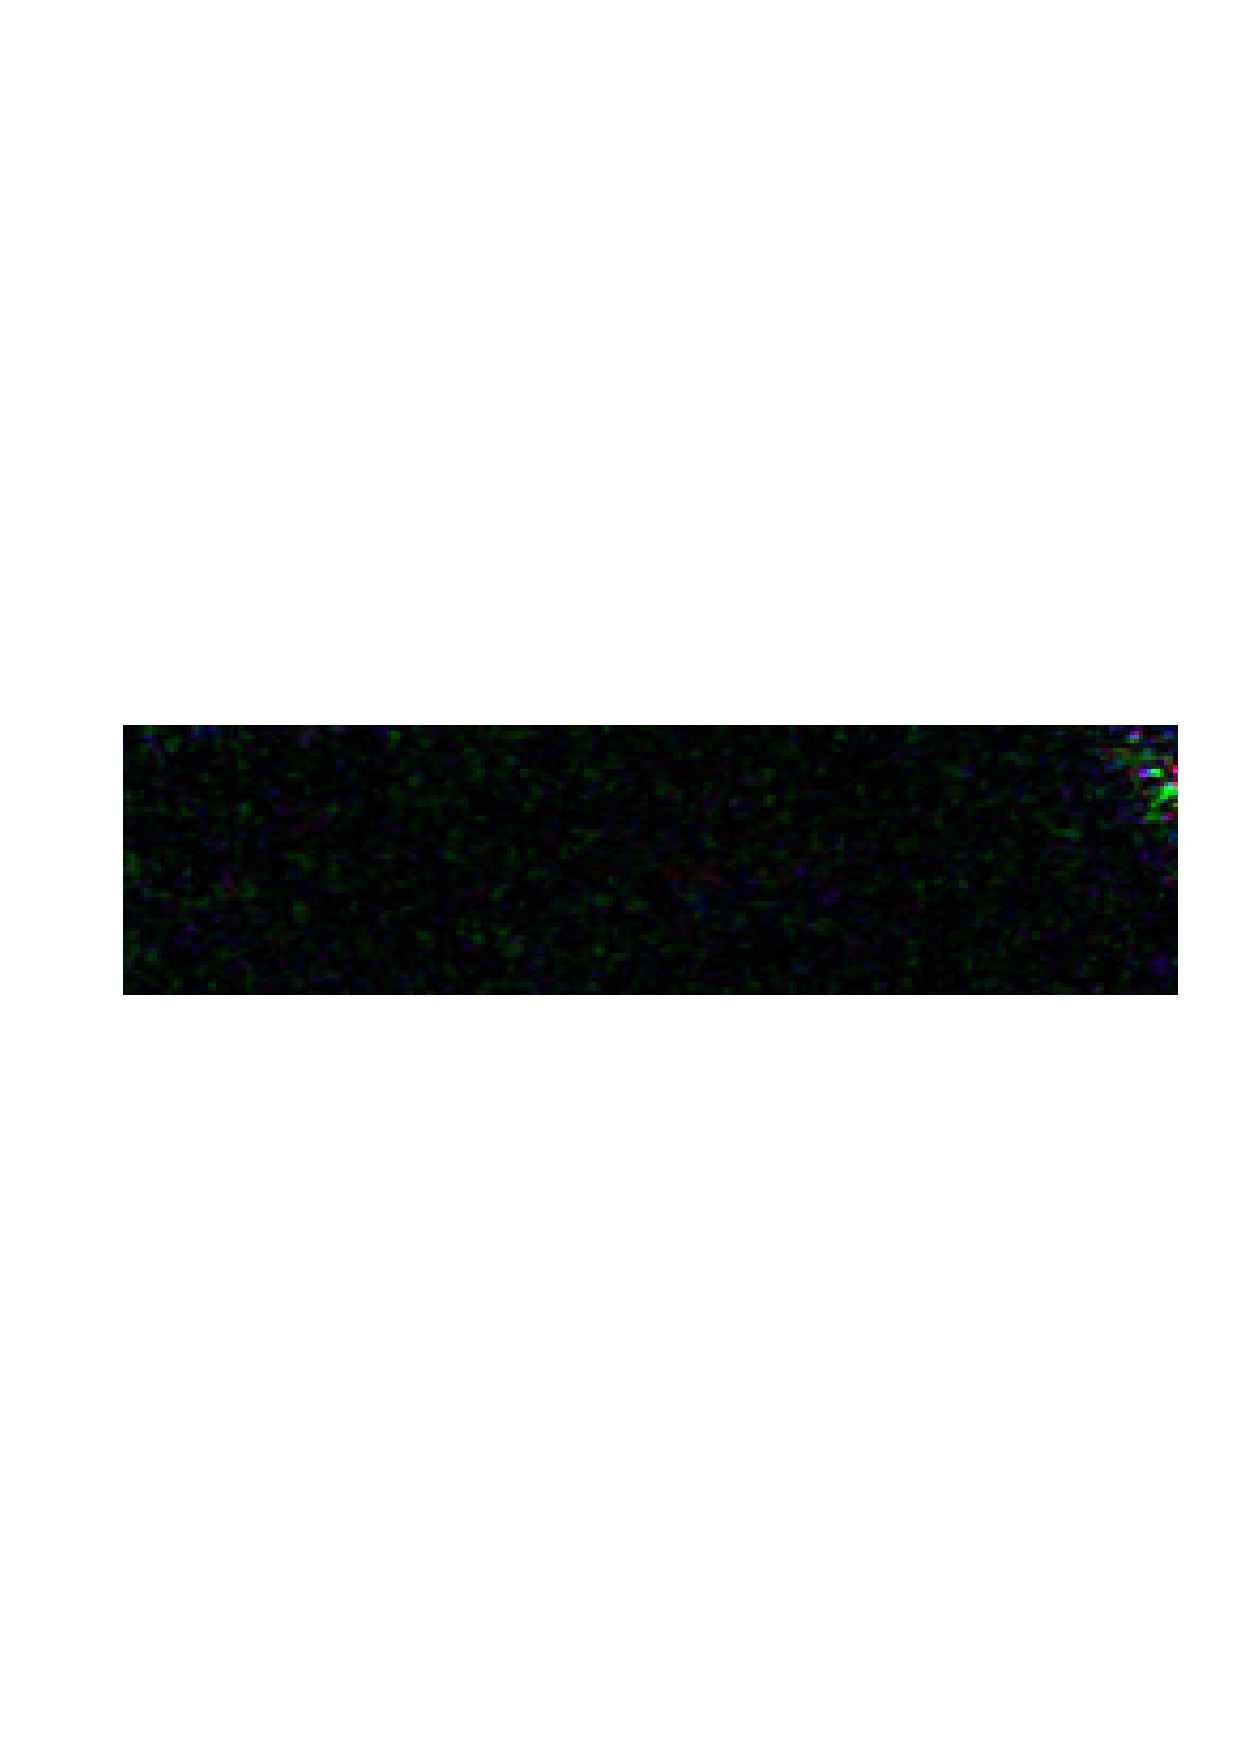
\includegraphics[width=.32\linewidth]{dark_linearized.pdf}}\ 
	\subfloat[Equalized \textit{dark} data\label{Fig:Equalized_dark}]{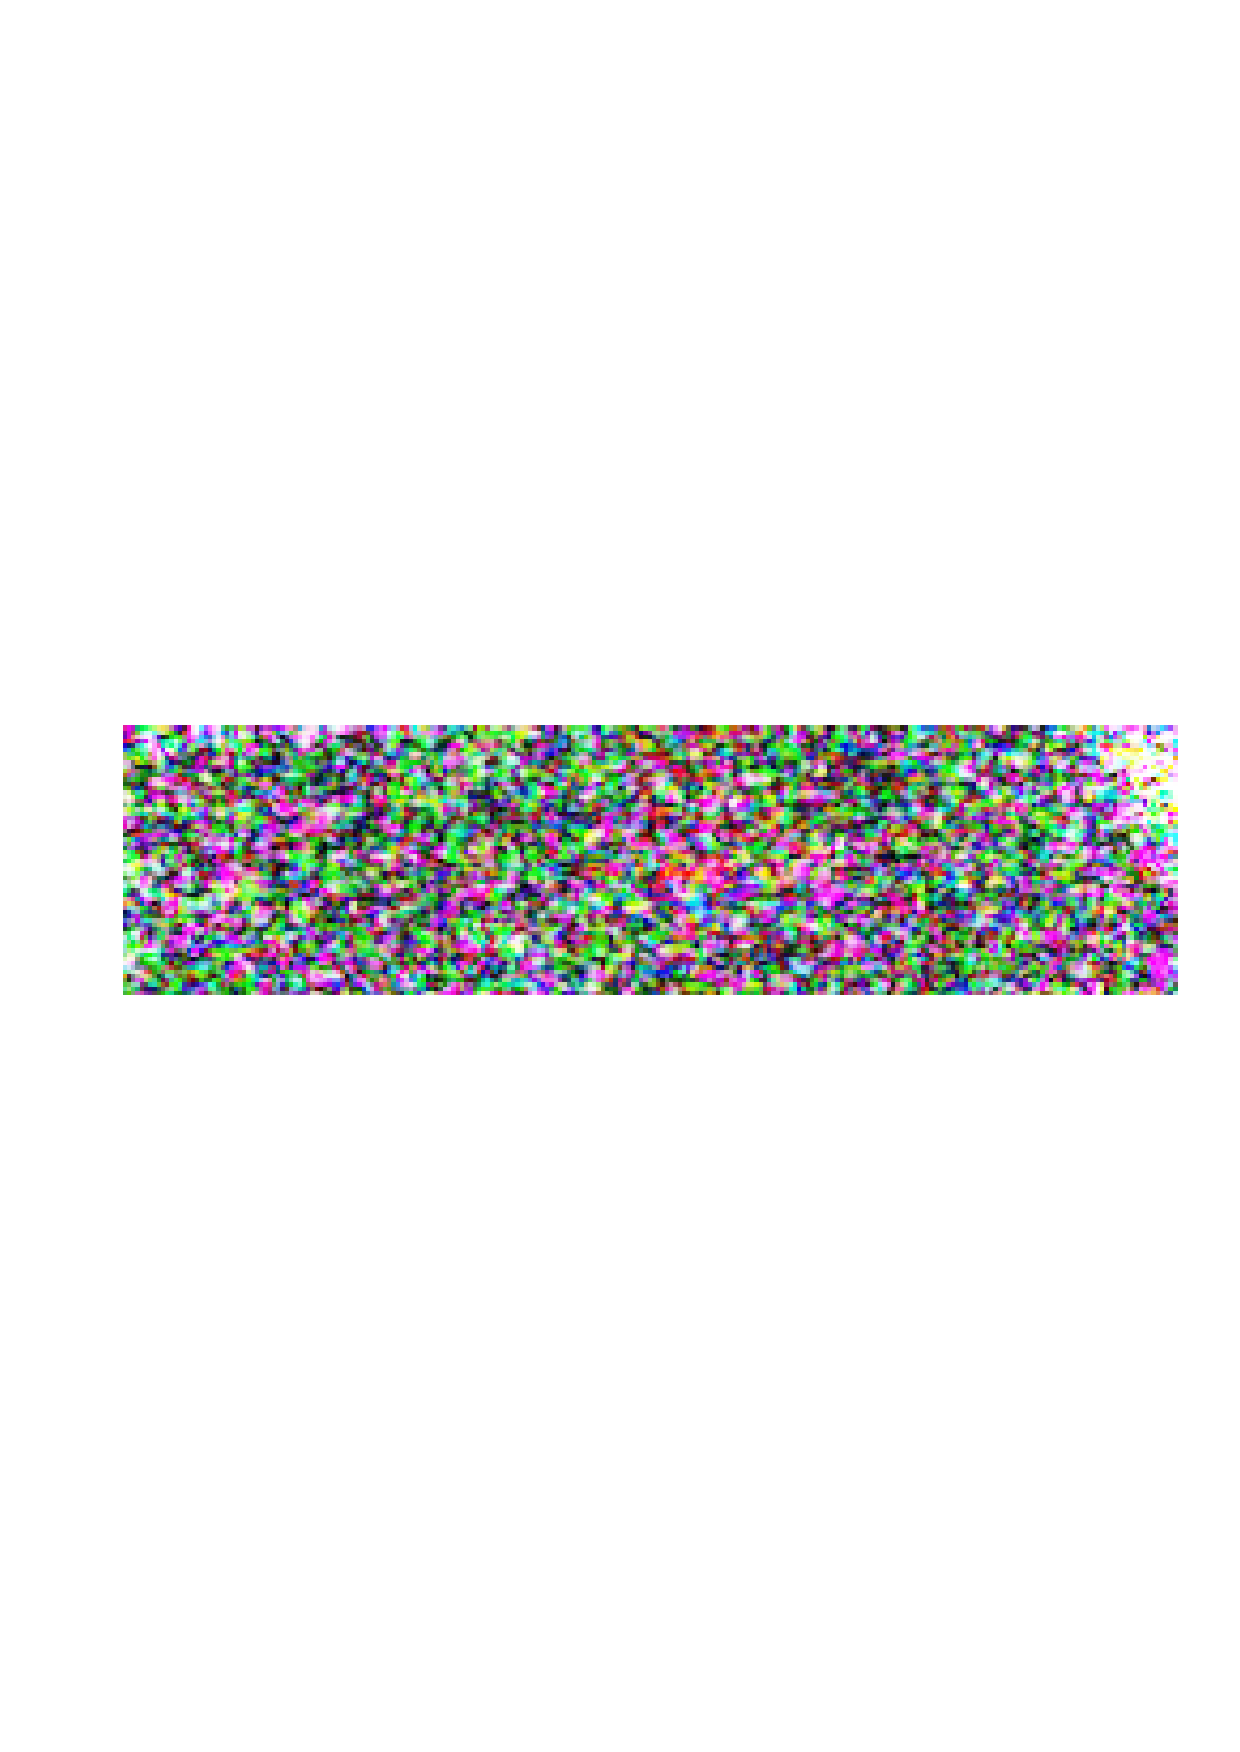
\includegraphics[width=.32\linewidth]{dark_equalized.pdf}}\ 
	\subfloat[\textit{dark} data with Beta histograms\label{Fig:BetaHistograms_dark}]{
\includegraphics[width=.32\linewidth]{dark_beta88.pdf}}
	\caption{Linearization, equalization and $\mathcal{B}(8,8)$ histogram stipulation of \textit{dark} data}
	\label{Fig:LiEqBe_dark}
\end{figure*}

\begin{figure*}[htb]
	\centering
	\subfloat[Linearized \textit{bright} data\label{Fig:Linearized_bright}]{
\includegraphics[width=.32\linewidth]{bright_linearized.pdf}}\ 
	\subfloat[Equalized \textit{bright} data\label{Fig:Equalized_bright}]{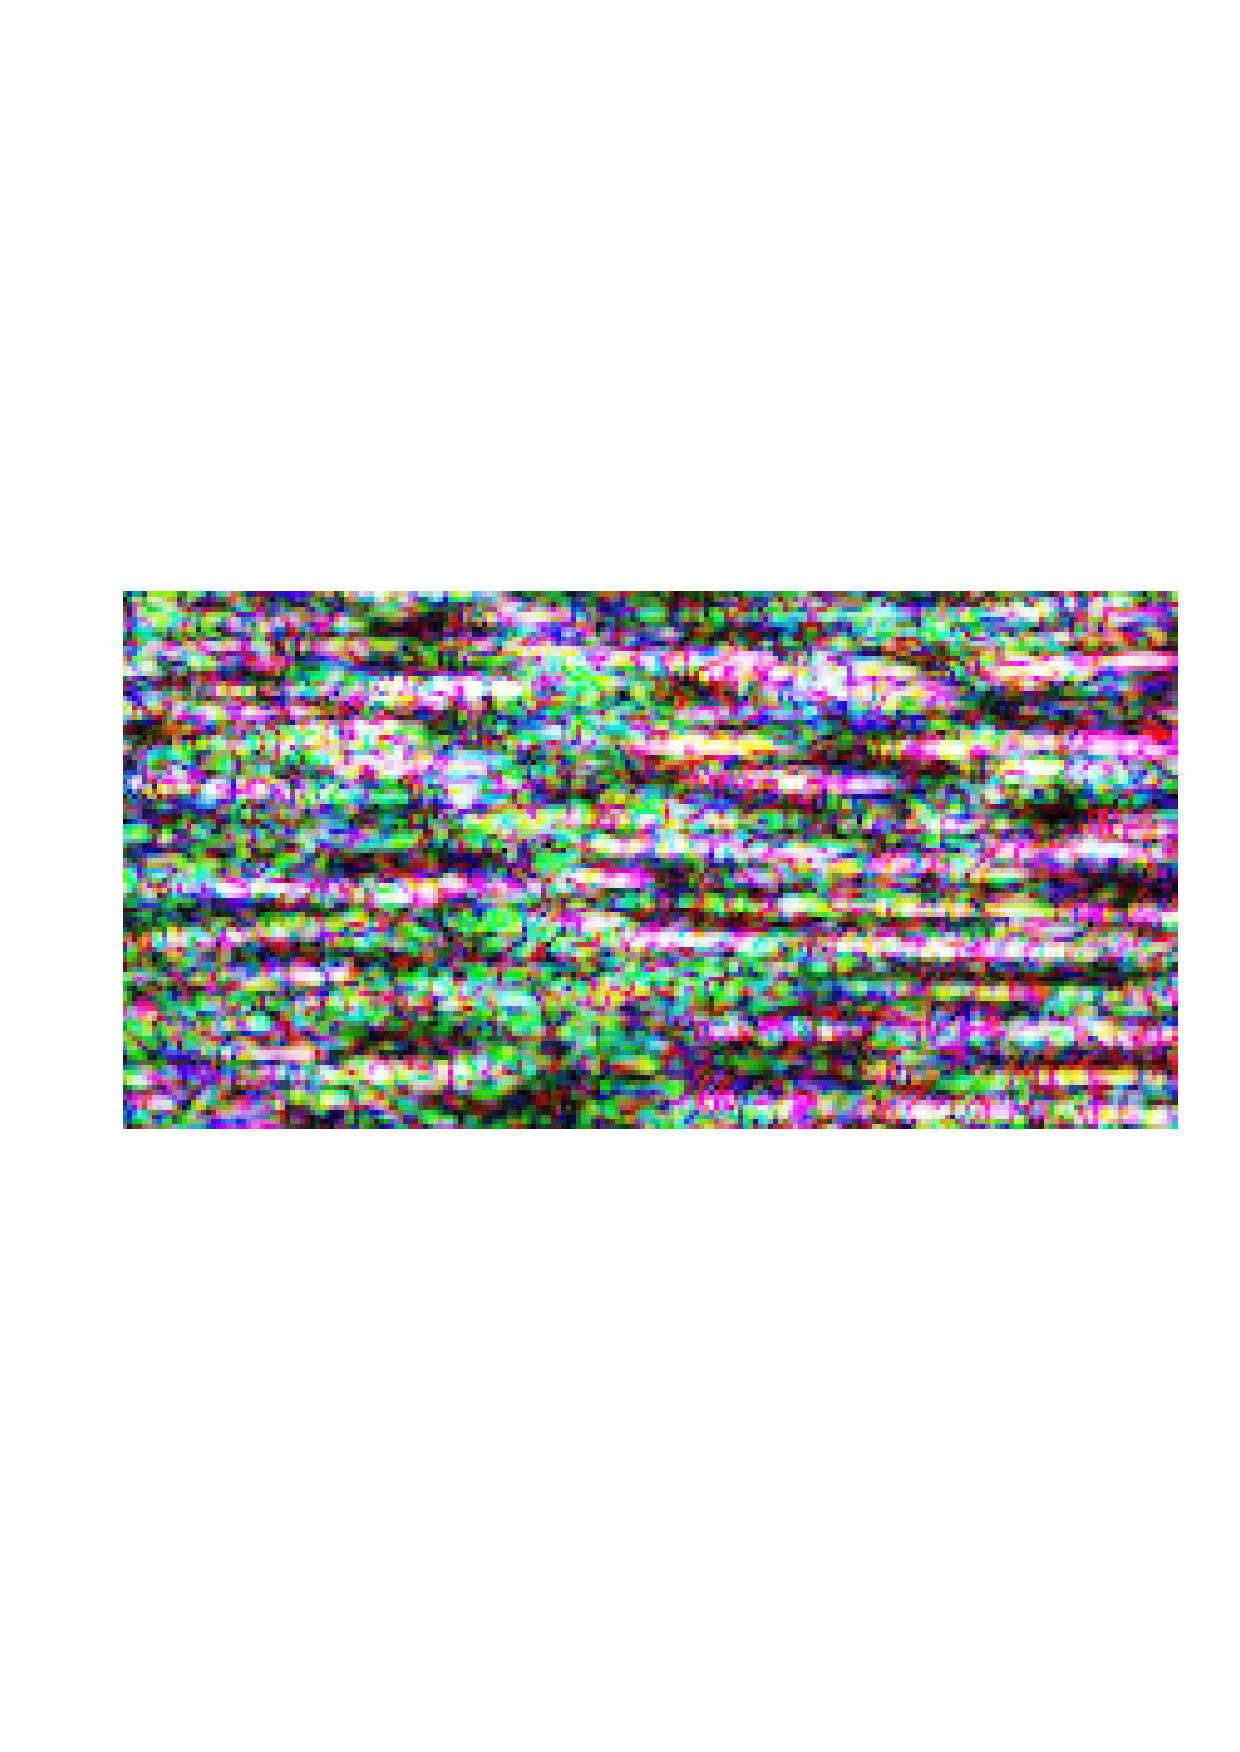
\includegraphics[width=.32\linewidth]{bright_equalized.pdf}}\ 
	\subfloat[\textit{bright} data with Beta histograms\label{Fig:BetaHistograms_bright}]{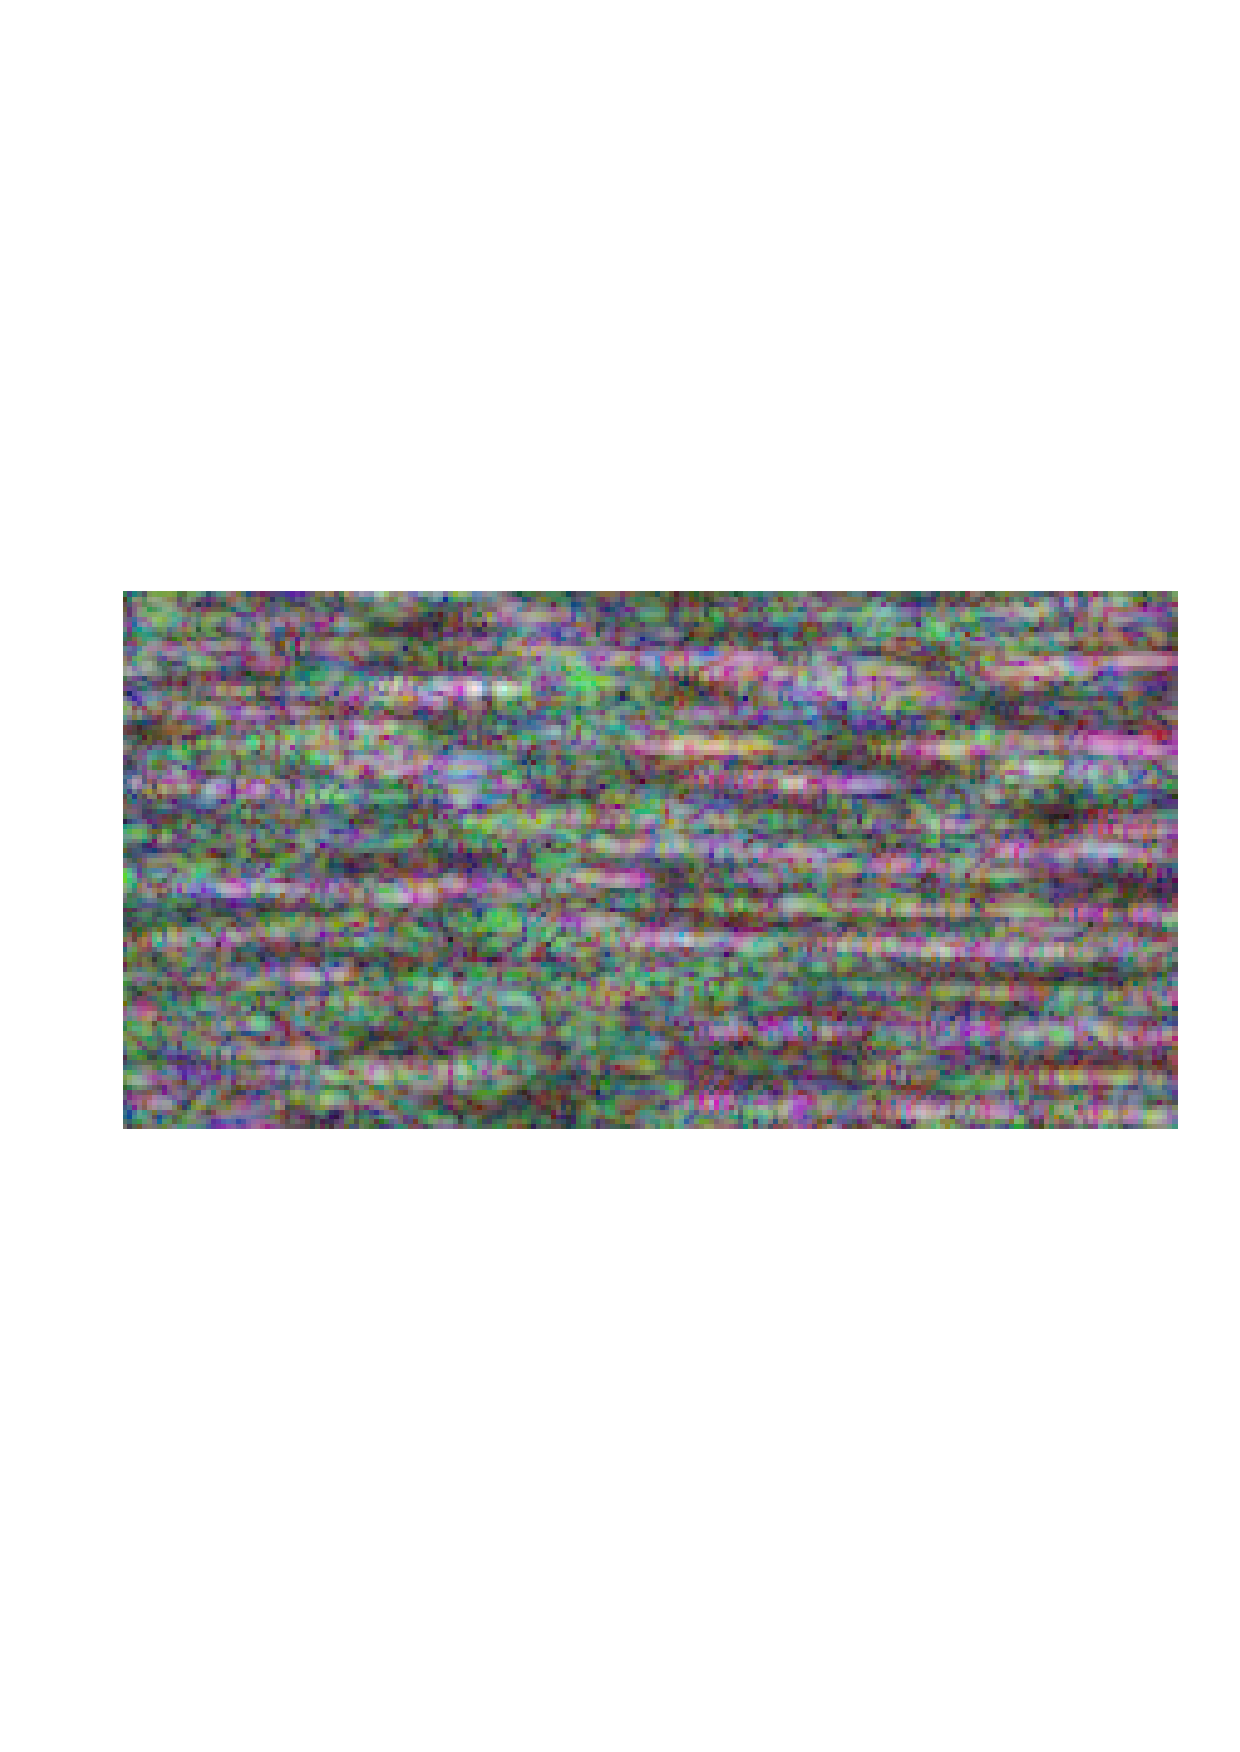
\includegraphics[width=.32\linewidth]{bright_beta88.pdf}}
	\caption{Linearization, equalization and $\mathcal{B}(8,8)$ histogram stipulation of \textit{bright} data}
	\label{Fig:LiEqBe_bright}
\end{figure*}

\newpage
Similar to Fig.\ref{Fig:LiEqBe_dark}, Fig.\ref{Fig:LiEqBe_bright} is the visualization of \textit{bright} data. For the sake of simplicity, I only show the codes(in Listing \ref{code:LiEqBe_dark}) corresponding to the \textit{dark} data.

\begin{lstlisting}[caption={Linearize, equalize and assign $\mathcal{B}(8,8)$ histogram to \textit{dark} data},label={code:LiEqBe_dark}]
# [dark] Linearized
plot(imagematrix(normalize_indep(dark)))

# [dark] Equalized
dark.equalize_indep <- c(ecdf(dark[,,1])(dark[,,1]),ecdf(dark[,,2])(dark[,,2]),ecdf(dark[,,3])(dark[,,3]))
plot(imagematrix(normalize_indep(array(dark.equalize_indep, dim=dim(dark)))))

# [dark] ~beta(8,8)
dark.beta.r <- qbeta(ecdf(dark[,,1])(dark[,,1]), shape1 = 8, shape2 = 8)
dark.beta.g <- qbeta(ecdf(dark[,,2])(dark[,,2]), shape1 = 8, shape2 = 8)
dark.beta.b <- qbeta(ecdf(dark[,,3])(dark[,,3]), shape1 = 8, shape2 = 8)
dark.beta_indep <- c(dark.beta.r,dark.beta.g,dark.beta.b)
plot(imagematrix((normalize_indep(array(dark.beta_indep, dim=dim(dark))))))
\end{lstlisting}


Then I try to specify the histogram as Beta distributions with different parameters. Fig.\ref{Fig:betas_dark} shows the histograms of each channel and the visualization of data specified as $\mathcal{B}(2,2), \mathcal{B}(8,8), \mathcal{B}(20,20)$ with the same mean. From histograms in Fig.\ref{Fig:betas_dark} we can see that the data specified as $\mathcal{B}(20,20)$ has more values clustered in a narrow range. Thus, the image looks smoother with lower contrast. While the data specified as $\mathcal{B}(2,2)$ is relatively evenly distributed, and the image has higher contrast. Fig.\ref{Fig:betas2_dark} shows the histograms and the visualization of data specified as $\mathcal{B}(20,4), \mathcal{B}(4,20)$. From histograms in Fig.\ref{Fig:betas2_dark} we can see that the data specified as $\mathcal{B}(20,4)$ has more values clustered in high interval while $\mathcal{B}(4,20)$ has more values clustered in low interval. Thus, the image of $\mathcal{B}(20,4)$ is brighter than the image of $\mathcal{B}(4,20)$.

For the sake of simplicity, here I only show the codes(in Listing \ref{code:hist_vis_beta22}) for drawing histograms and visualizing the data specified as $\mathcal{B}(2,2)$.

\begin{lstlisting}[caption={Drawing histograms and visualizing the data specified as $\mathcal{B}(2,2)$},label={code:hist_vis_beta22}]
# Assign Beta(2,2) to each channel
dark.beta_2_2.r <- qbeta(ecdf(dark[,,1])(dark[,,1]), shape1 = 2, shape2 = 2)
dark.beta_2_2.g <- qbeta(ecdf(dark[,,2])(dark[,,2]), shape1 = 2, shape2 = 2)
dark.beta_2_2.b <- qbeta(ecdf(dark[,,3])(dark[,,3]), shape1 = 2, shape2 = 2)
dark.beta_2_2_indep <- c(dark.beta_2_2.r,dark.beta_2_2.g,dark.beta_2_2.b)

# Draw histograms of each channel
hist(dark.beta_2_2.r,probability = TRUE, breaks = "FD")
hist(dark.beta_2_2.g,probability = TRUE, breaks = "FD")
hist(dark.beta_2_2.b,probability = TRUE, breaks = "FD")

# Visualize the image
plot(imagematrix((normalize_indep(array(dark.beta_2_2_indep, dim=dim(dark))))))
\end{lstlisting}

\begin{figure}[htbp]
	\centering
	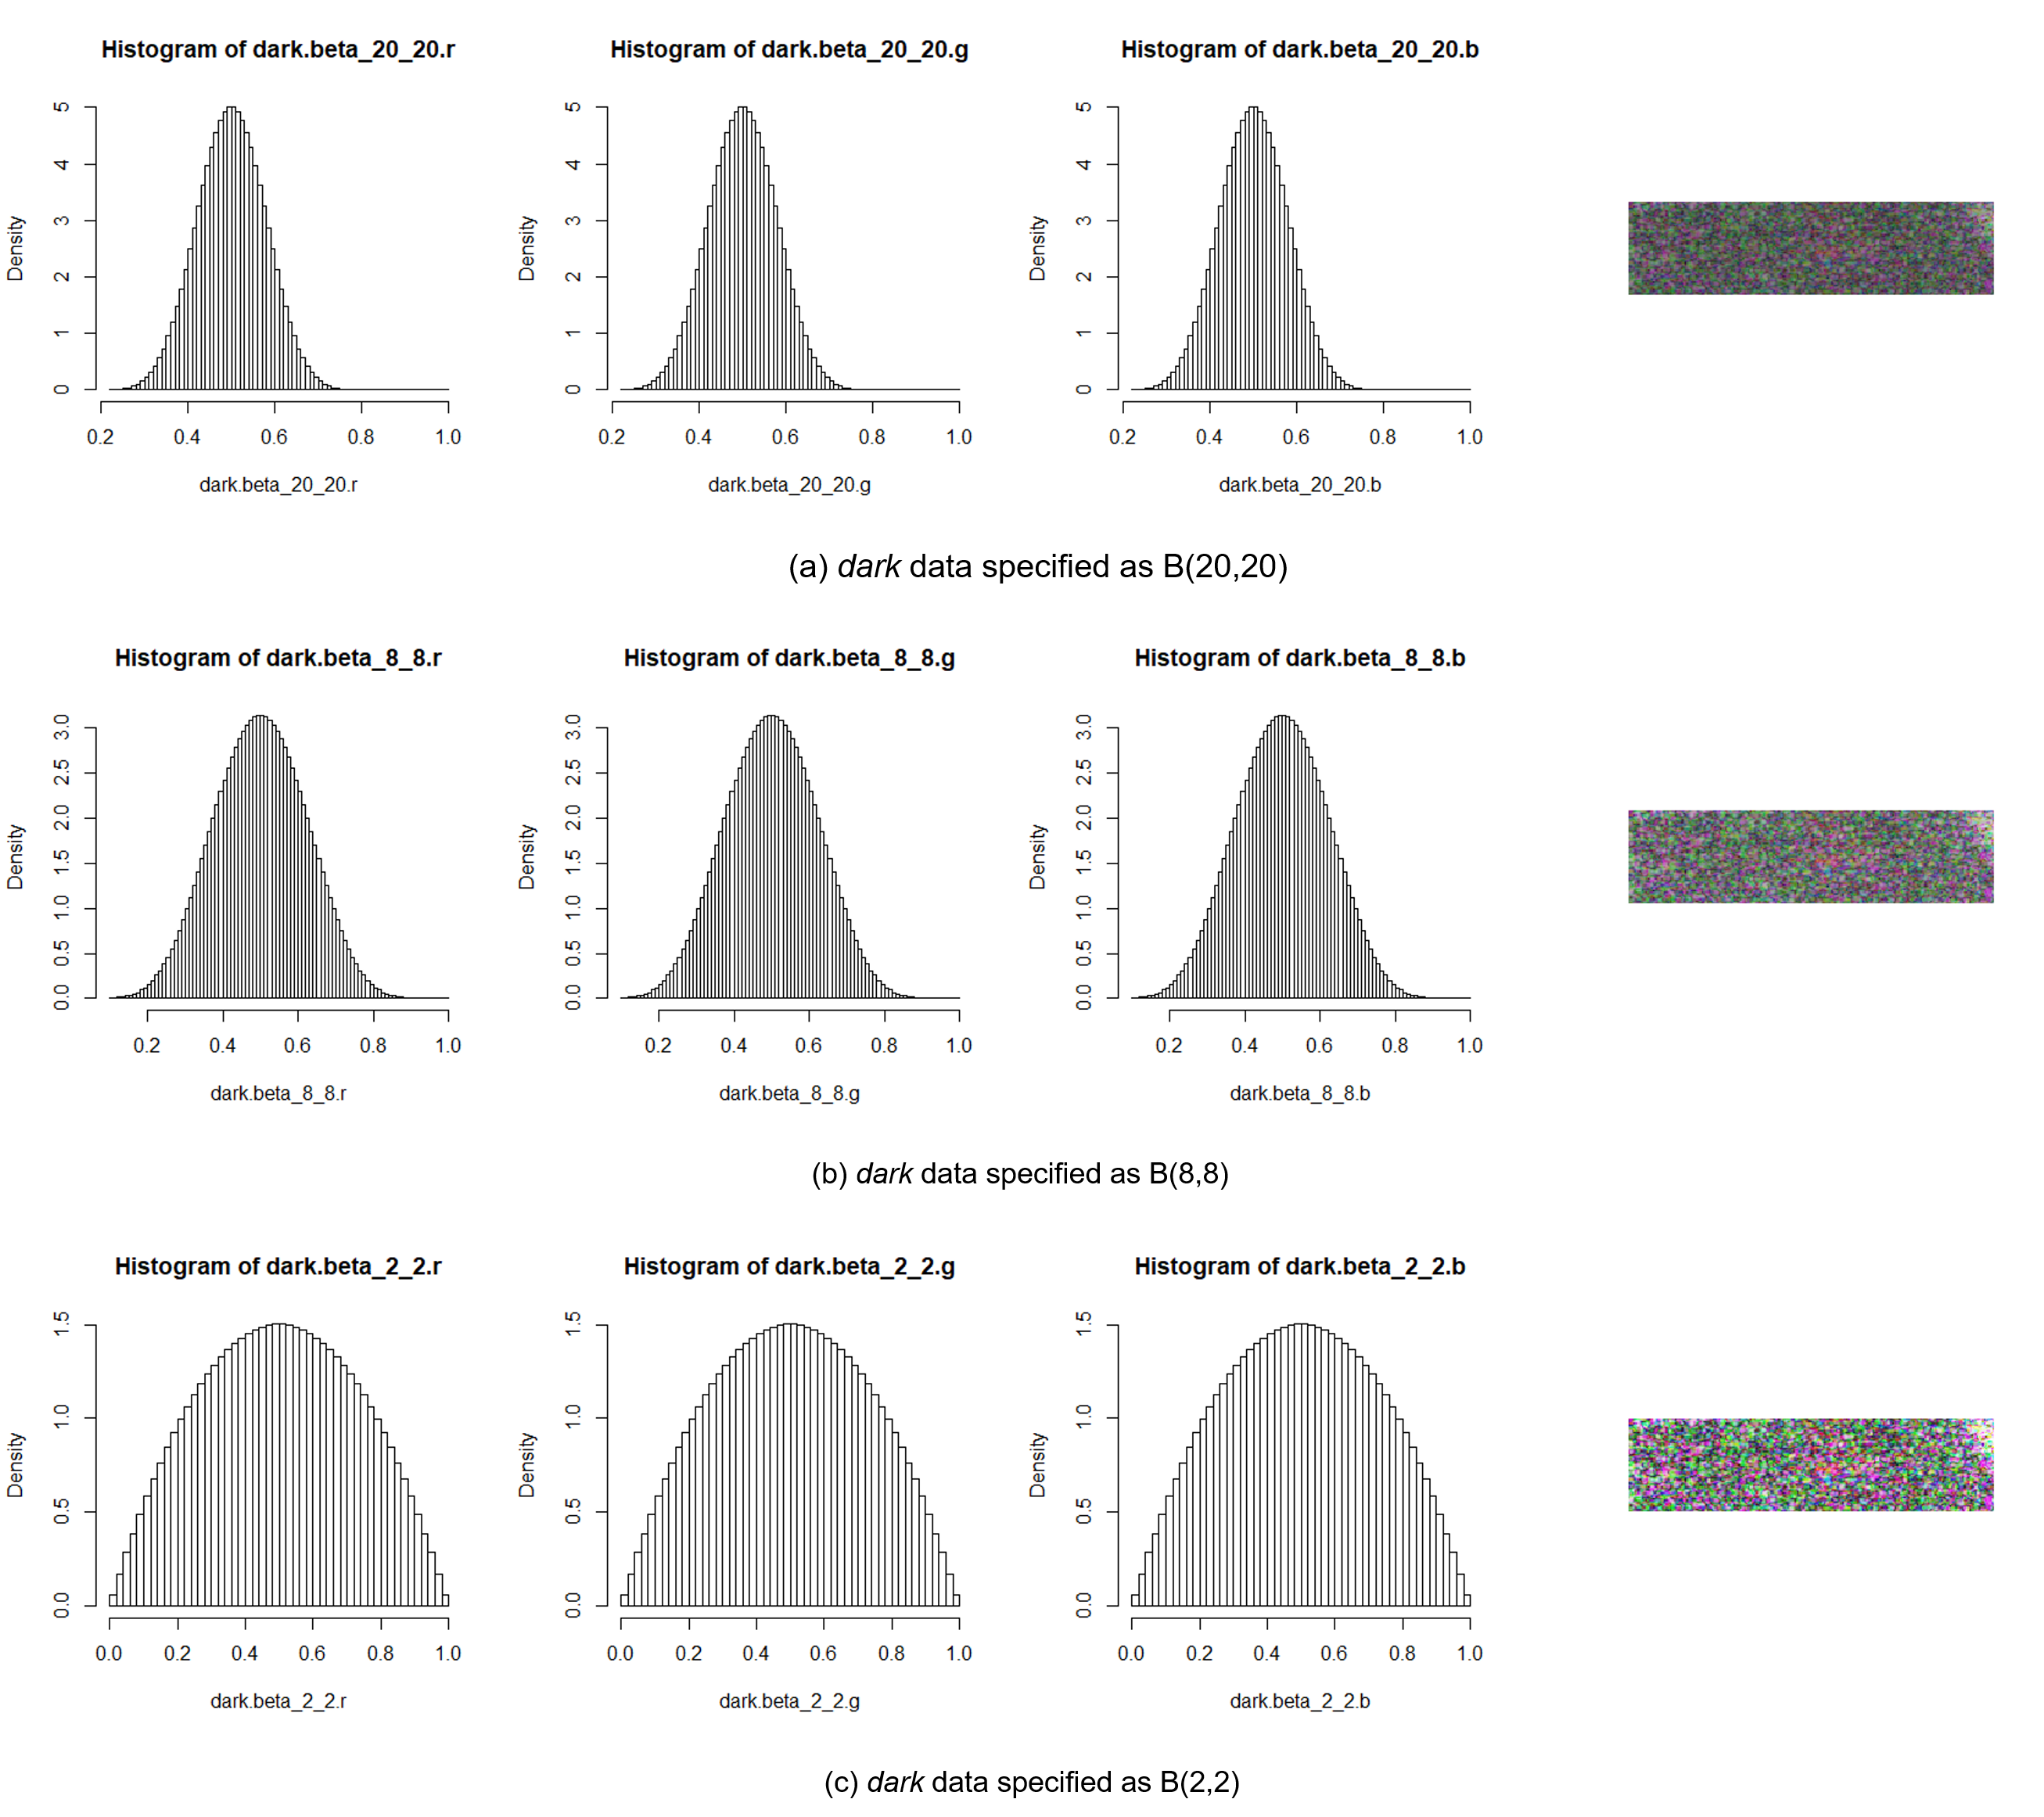
\includegraphics[width=\linewidth]{betas_dark.png}
	\caption{Histograms and image of \textit{dark} data specified as $\mathcal{B}(2,2), \mathcal{B}(8,8), \mathcal{B}(20,20)$}
	\label{Fig:betas_dark}
\end{figure}

\begin{figure}[htbp]
	\centering
	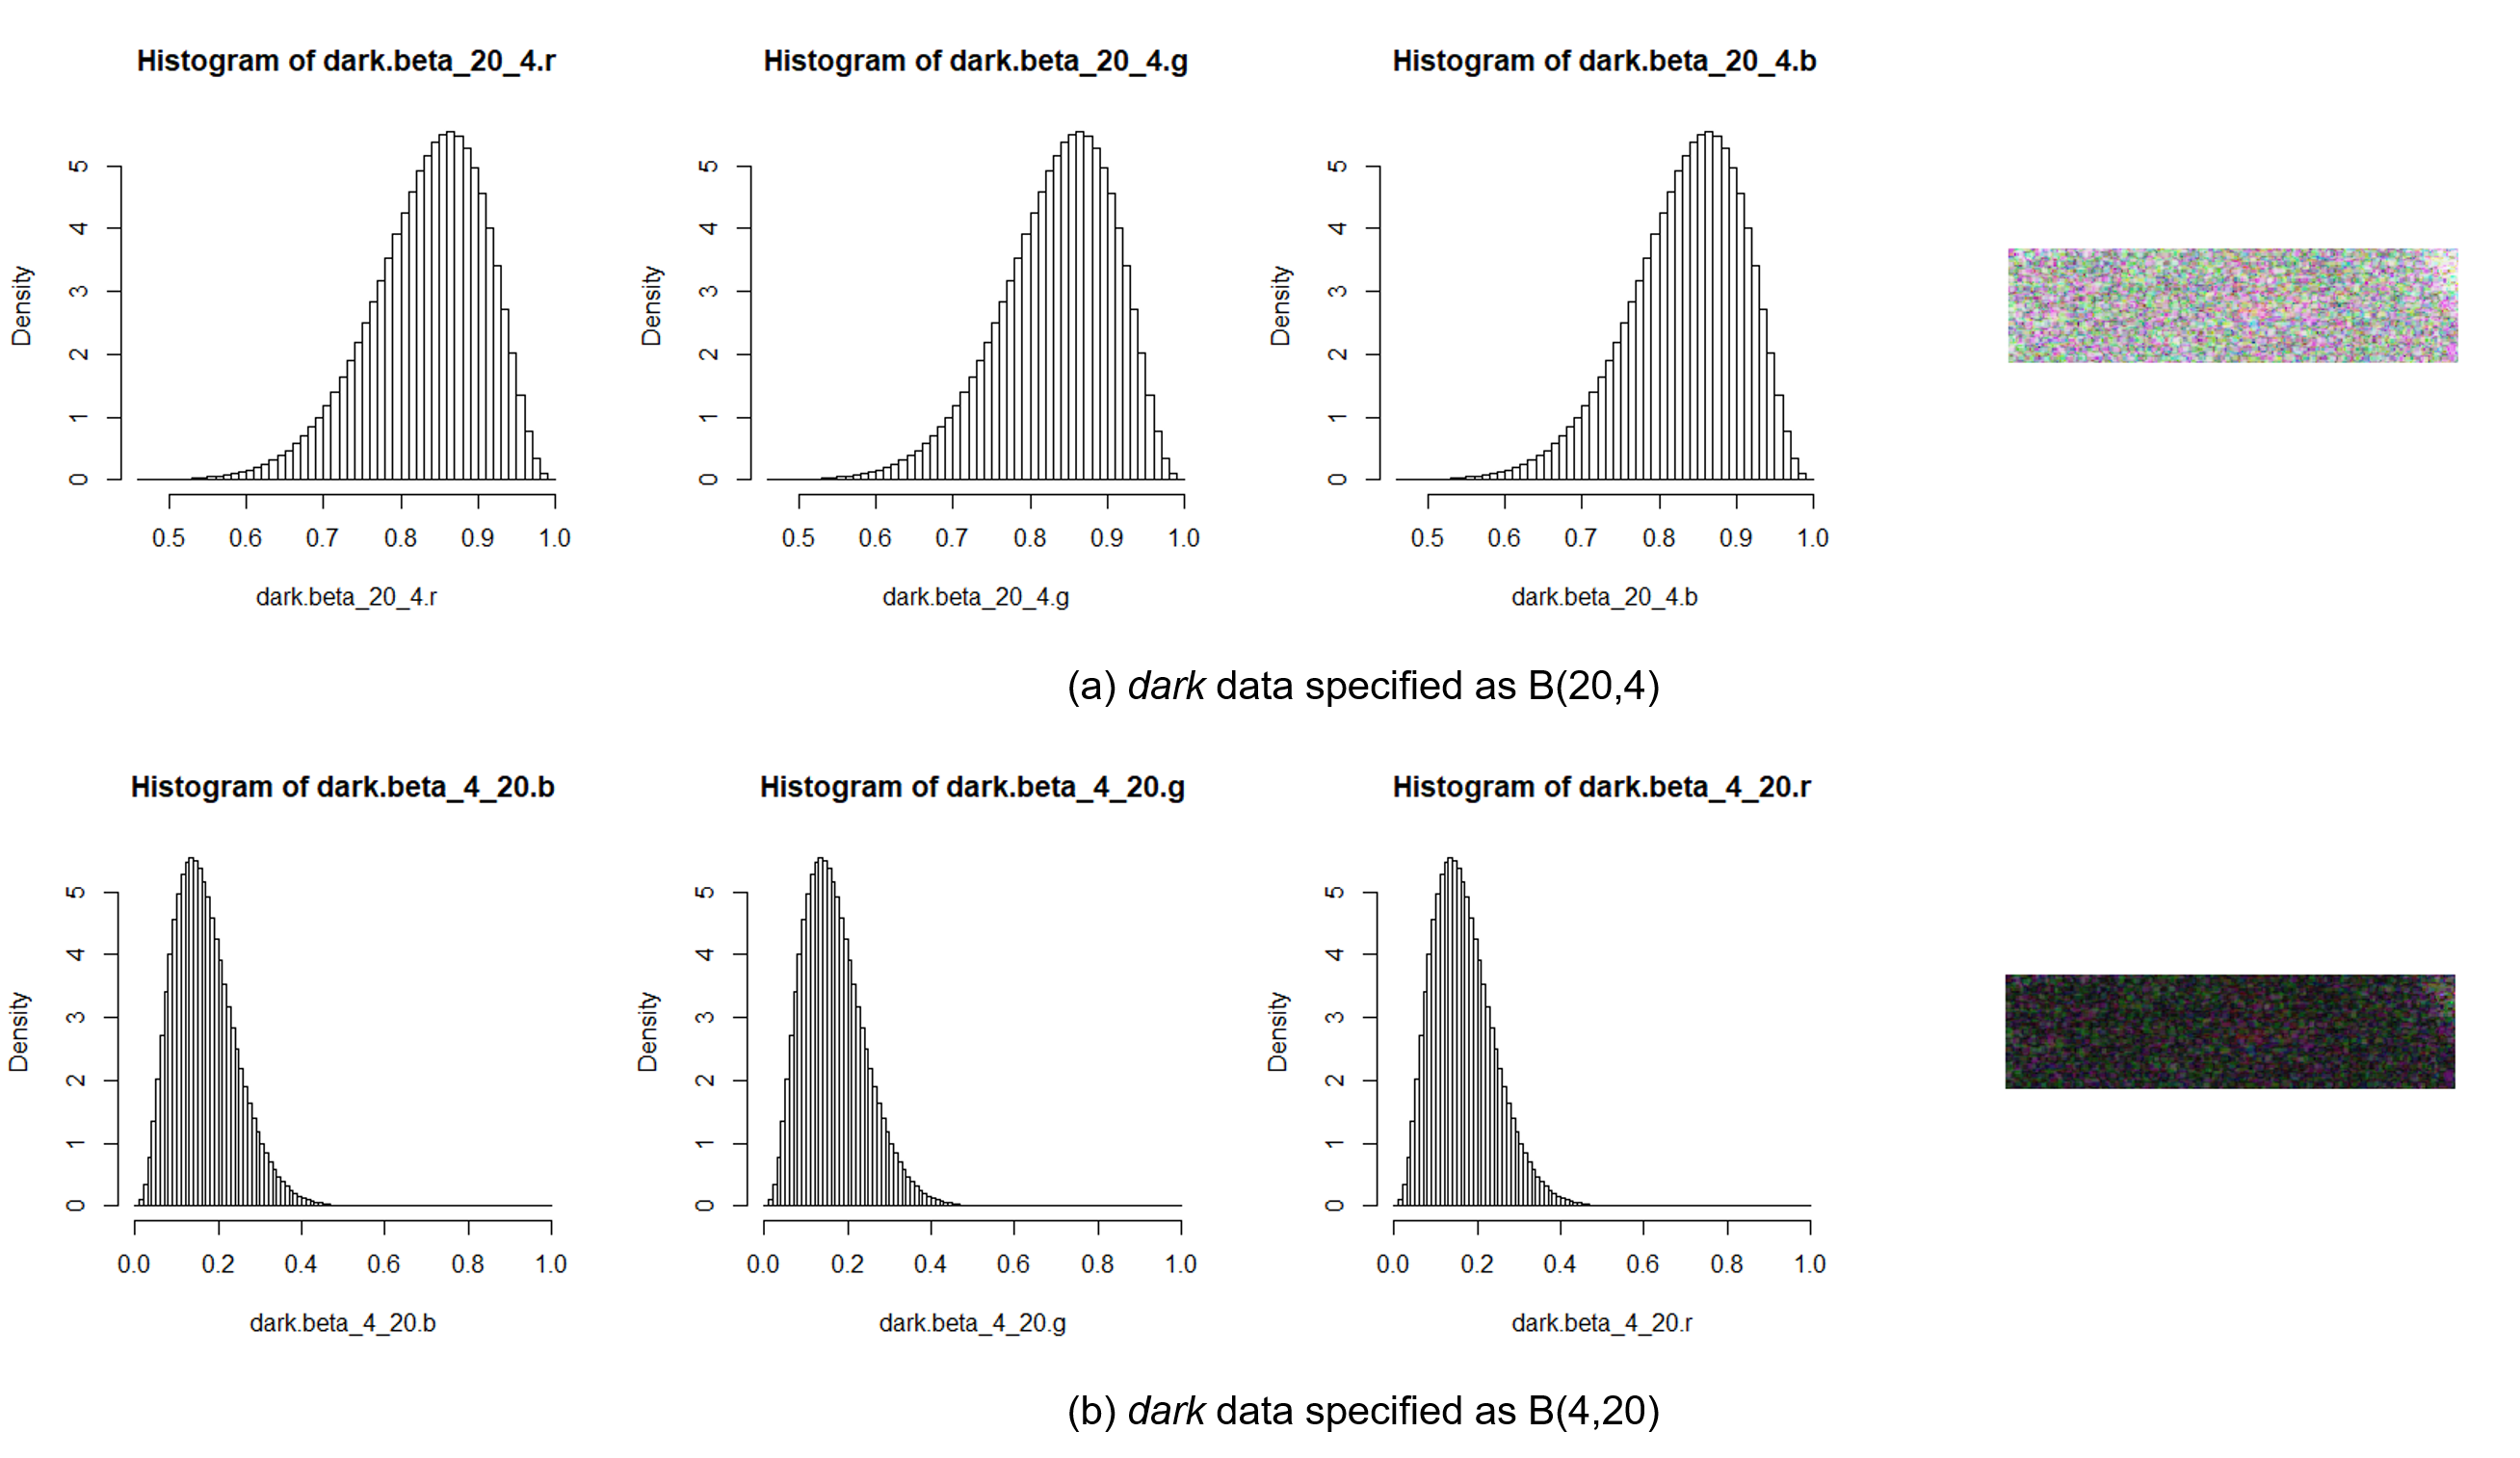
\includegraphics[width=\linewidth]{betas2_dark.png}
	\caption{Histograms and image of \textit{dark} data specified as $\mathcal{B}(20,4), \mathcal{B}(4,20)$}
	\label{Fig:betas2_dark}
\end{figure}


\newpage
\section{Assignment 3 (2019-07-17)}
\subsection{Define and call functions}

In this part, We define several functions and then call the functions we defined to plot them. The code is shown in Listing \ref{code:functions} and in Fig.\ref{Fig:funcs} we plot the functions. Interestingly, Fig.\ref{Fig:sin1s} shows $f(x)=xsin(\frac{1}{x})$ over different ranges of x, where we can see that function $f(x)=xsin(\frac{1}{x})$ oscillates more and more rapidly when x gets closer to 0, and its amplitude reduces.

\begin{lstlisting}[caption={Define and call functions},label={code:functions}]
# Define the functions
f.square <- function(x){
x^2
}
f.power <- function(x,a){
x^a
}
f.sin1 <- function(x){
x*sin(1/x)
}

# Call and plot the functions
x <- seq(-10^-2,10^-2,length.out = 10000)
plot(x,f.square(x),type="l",col="black")
plot(x,f.power(x,3),type="l",col="blue")
plot(x,f.sin1(x),type="l",col="red")
\end{lstlisting}

\begin{figure*}[htbp]
	\centering
	\subfloat[f.square(x)=$x^2$ \label{Fig:f_square}]{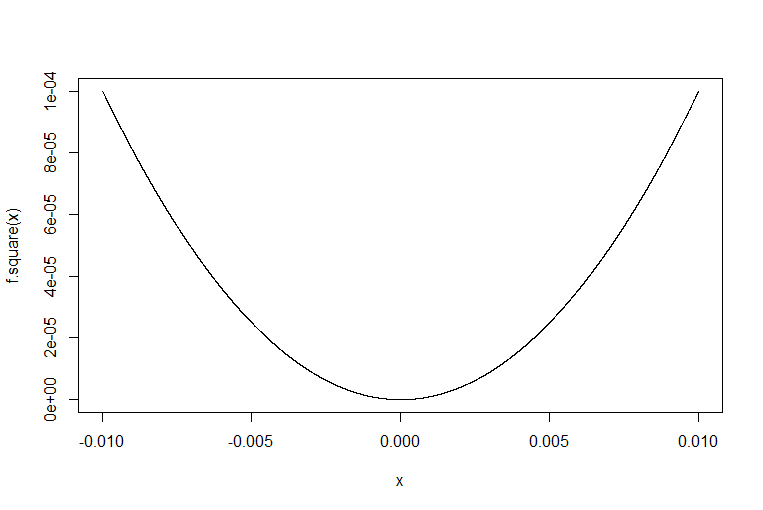
\includegraphics[width=.3\linewidth]{f_square.png}}\ 
	\subfloat[f.power(x,3)=$x^3$ \label{Fig:f_power}]{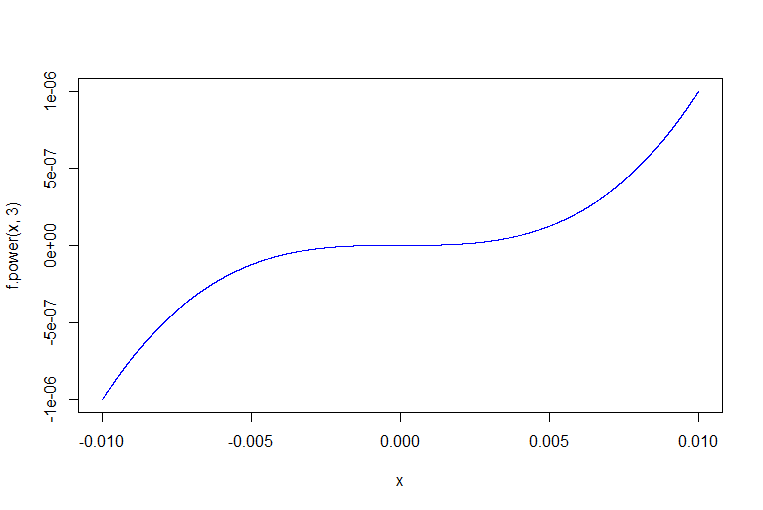
\includegraphics[width=.3\linewidth]{f_power.png}}\
	\subfloat[f.sin1(x)=$xsin(\frac{1}{x})$ \label{Fig:f_sin1}]{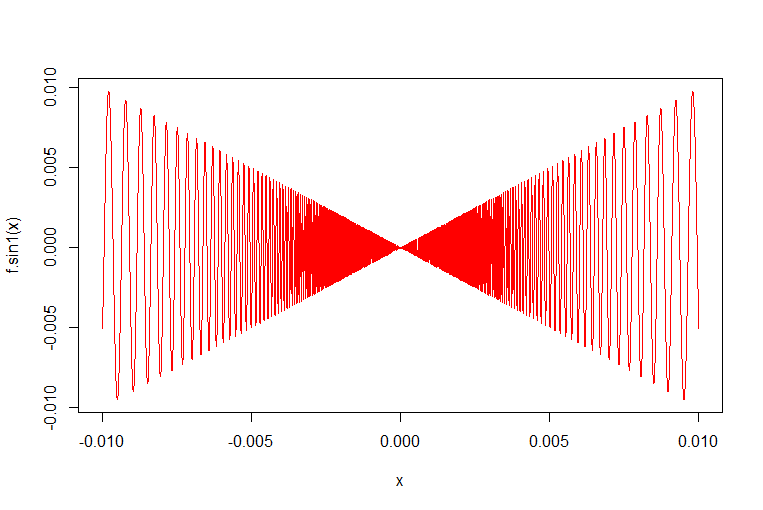
\includegraphics[width=.3\linewidth]{f_sin1.png}}\   
	\caption{Plot the functions}
	\label{Fig:funcs}
\end{figure*}

\begin{figure*}[htbp]
	\centering
	\subfloat[$x\in(-1,1)$ \label{Fig:sin1_1}]{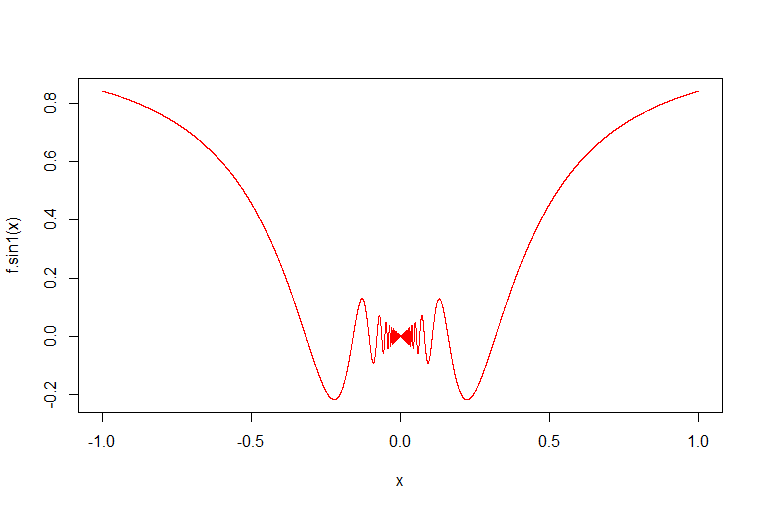
\includegraphics[width=.3\linewidth]{sin1_1.png}}\ 
	\subfloat[$x\in(-0.01,0.01)$ \label{Fig:sin1_2}]{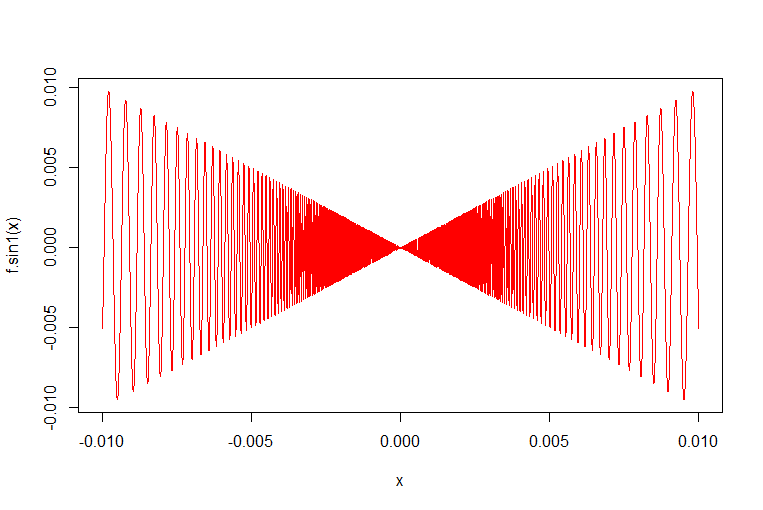
\includegraphics[width=.3\linewidth]{sin1_2.png}}\
	\subfloat[$x\in(-10^{-5},10^{-5})$ \label{Fig:sin1_3}]{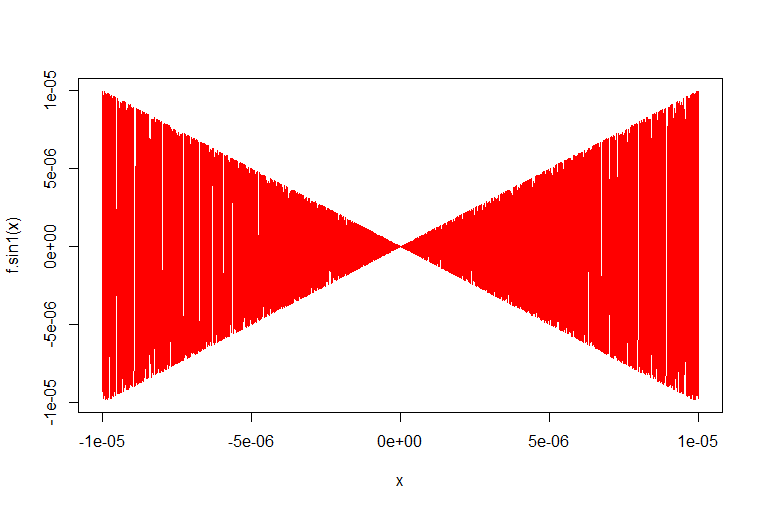
\includegraphics[width=.3\linewidth]{sin1_3.png}}\   
	\caption{$f(x)=xsin(\frac{1}{x})$ over different ranges of x }
	\label{Fig:sin1s}
\end{figure*}


\subsection{Implement $\mathcal{K}$ distribution with R}

Fig.\ref{Fig:K_dis_alpha} shows the densities in linear and semilogarithmic scale of $\mathcal{K}$ distribution with L=1, and black, red, blue curves are for $\alpha\in\{2,5,10\}$, respectively. To learn the effects of varying $\alpha$, we show  $\mathcal{K}$ distributions with the same unitary mean. From the results we can see that when L is fixed, the smaller the value of $\alpha$ is, the higher contrast the data has, that is smaller $\alpha$ assigns larger probabilities to both small and large values. $\alpha$ is related to the number of elementary backscatterers. When the value of $\alpha$ is large, the density of $\mathcal{K}$ distribution is close to the density of exponential distribution.

Fig.\ref{Fig:K_dis_L} shows the densities in linear and semilogarithmic scale of $\mathcal{K}$ distribution with $\alpha=2, \lambda=2$, and black, red, blue curves are for $L\in\{1,4,7\}$, respectively. As shown in Fig.\ref{Fig:K_dis_L}, when $\alpha$ and $\lambda$ is fixed, the larger the value of looks $L$ is, the lower contrast the data has.

\begin{lstlisting}[caption={$\mathcal{K}$ distribution}]
# K distribution PDF
f.K_dis <- function(x,alpha,lambda,L){
2*lambda*L/(gamma(alpha)*gamma(L))*((lambda*L*x)^((alpha+L)/2-1))*besselK(2*sqrt(lambda*L*x),alpha-L)
}

x <- seq(0,8,length.out = 1000)

## K distribution with L=1 alpha in {2,5,10}
plot(x,f.K_dis(x,2,2,1),type="l",col="black")
lines(x,f.K_dis(x,5,5,1),col="red")
lines(x,f.K_dis(x,10,10,1),col="blue")
# semilog scale
plot(x,f.K_dis(x,2,2,1),type="l",col="black",log = "y")
lines(x,f.K_dis(x,5,5,1),col="red")
lines(x,f.K_dis(x,10,10,1),col="blue")

## K distribution with alpha=2 lambda=2  L in {1,4,7}
plot(x,f.K_dis(x,2,2,1),type="l",col="black")
lines(x,f.K_dis(x,2,2,4),col="red")
lines(x,f.K_dis(x,2,2,7),col="blue")
# semilog scale
plot(x,f.K_dis(x,2,2,1),type="l",col="black", log = "y")
lines(x,f.K_dis(x,2,2,4),col="red")
lines(x,f.K_dis(x,2,2,7),col="blue")
\end{lstlisting}

\begin{figure*}[htb]
	\centering
	\subfloat[L=1 Densities \label{Fig:K_alpha}]{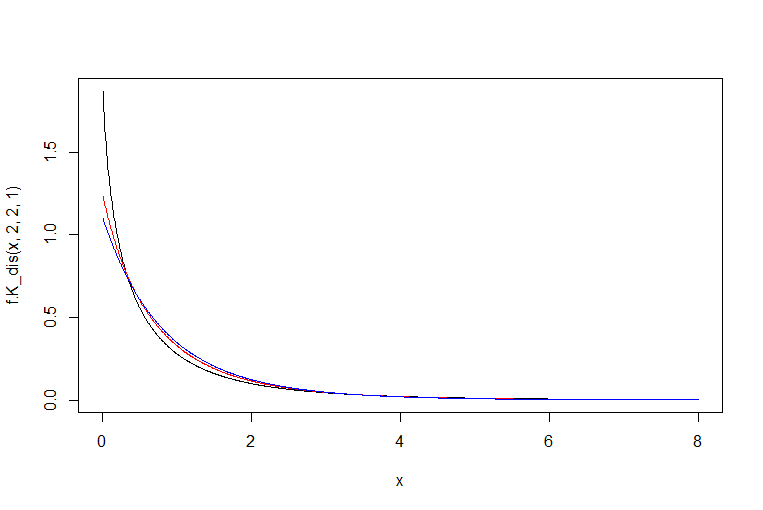
\includegraphics[width=.45\linewidth]{K_alpha.png}}\ 
	\subfloat[L=1 Densities in semilog scale \label{Fig:K_alpha_semilog}]{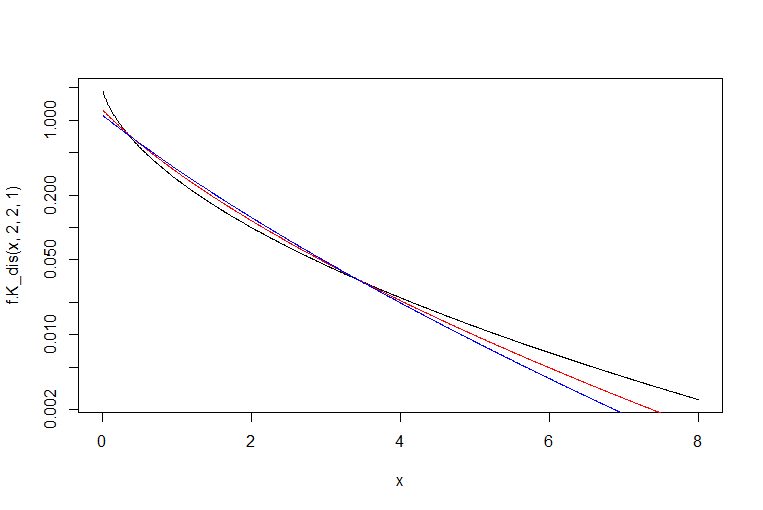
\includegraphics[width=.45\linewidth]{K_alpha_semilog.png}}\ 
	\caption{Densities in linear and semilogarithmic scale of $\mathcal{K}$ distribution with unitary mean and L=1. Black, red, blue for $\alpha\in\{2,5,10\}$, respectively.}
	\label{Fig:K_dis_alpha}
\end{figure*}

\begin{figure*}[htb]
	\centering
	\subfloat[$\alpha=2,\lambda=2$ Densities \label{Fig:K_L}]{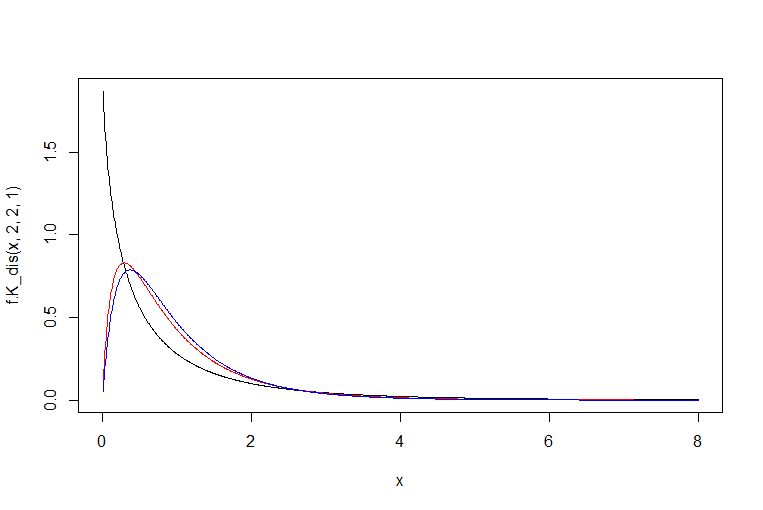
\includegraphics[width=.45\linewidth]{K_L.png}}\ 
	\subfloat[$\alpha=2,\lambda=2$ Densities in semilog scale \label{Fig:K_L_semilog}]{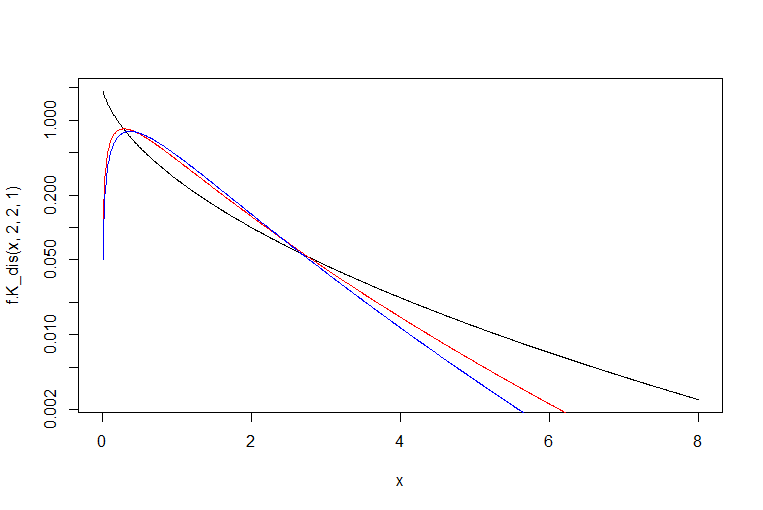
\includegraphics[width=.45\linewidth]{K_L_semilog.png}}\ 
	\caption{Densities in linear and semilogarithmic scale of $\mathcal{K}$ distribution with unitary mean and $\alpha=2,\lambda=2$. Black, red, blue for $L\in\{1,4,7\}$, respectively.}
	\label{Fig:K_dis_L}
\end{figure*}


\subsection{Implement $\mathcal{G}^0$ distribution with R}

Fig.\ref{Fig:G_dis_alpha} shows the densities in linear and semilogarithmic scale of $\mathcal{G}^0$ distribution with L=1, and black, red, blue curves are for $\alpha\in\{-2,-4,-10\}$, respectively. To learn the effects of varying $\alpha$, we show  $\mathcal{G}^0$ distributions with the same unitary mean. From the results we can see that when L is fixed, the larger the value of $\alpha$ is, the higher contrast the data has.

Fig.\ref{Fig:G_dis_L} shows the densities in linear and semilogarithmic scale of $\mathcal{G}^0$ distribution with $\alpha=-2, \gamma=1$, and black, red, blue curves are for $L\in\{1,3,5\}$, respectively. As shown in Fig.\ref{Fig:K_dis_L}, when $\alpha$ and $\gamma$ is fixed, the larger the value of looks $L$ is, the lower contrast the data has, which is similar to the $\mathcal{K}$ distribution.

\begin{lstlisting}[caption={$\mathcal{G}^0$ distribution}]
# GI0 distribution PDF
f.GI0_dis <- function(x,alpha,g,L){
L^L*(gamma(L-alpha))/(g^alpha*gamma(L)*gamma(-alpha))*x^(L-1)/((g+L*x)^(L-alpha))
}

x <- seq(0,8,length.out = 1000)

## GI0 distribution with L=1 alpha in {-2,-4,-10}
plot(x,f.GI0_dis(x,-2,1,1),type="l",col="black")
lines(x,f.GI0_dis(x,-4,3,1),col="red")
lines(x,f.GI0_dis(x,-10,9,1),col="blue")
# semilog scale
plot(x,f.GI0_dis(x,-2,1,1),type="l", col="black", log="y")
lines(x,f.GI0_dis(x,-4,3,1),col="red")
lines(x,f.GI0_dis(x,-10,9,1),col="blue")

## GI0 distribution with alpha=-2 g=1  L in {1,3,5}
plot(x,f.GI0_dis(x,-2,1,1),type="l", col="black")
lines(x,f.GI0_dis(x,-2,1,3),col="red")
lines(x,f.GI0_dis(x,-2,1,5),col="blue")
# semilog scale
plot(x,f.GI0_dis(x,-2,1,1),type="l", col="black", log="y")
lines(x,f.GI0_dis(x,-2,1,3),col="red")
lines(x,f.GI0_dis(x,-2,1,5),col="blue")

\end{lstlisting}

\begin{figure*}[htb]
	\centering
	\subfloat[L=1 Densities \label{Fig:G_alpha}]{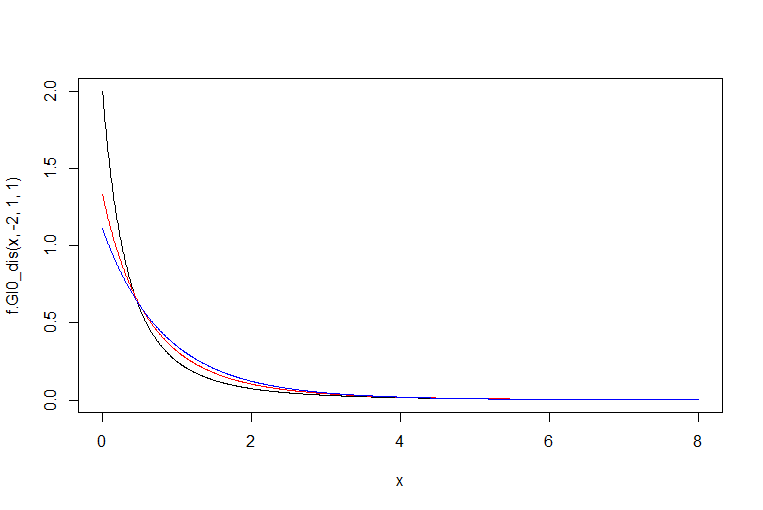
\includegraphics[width=.45\linewidth]{G_alpha.png}}\ 
	\subfloat[L=1 Densities in semilog scale \label{Fig:G_alpha_semilog}]{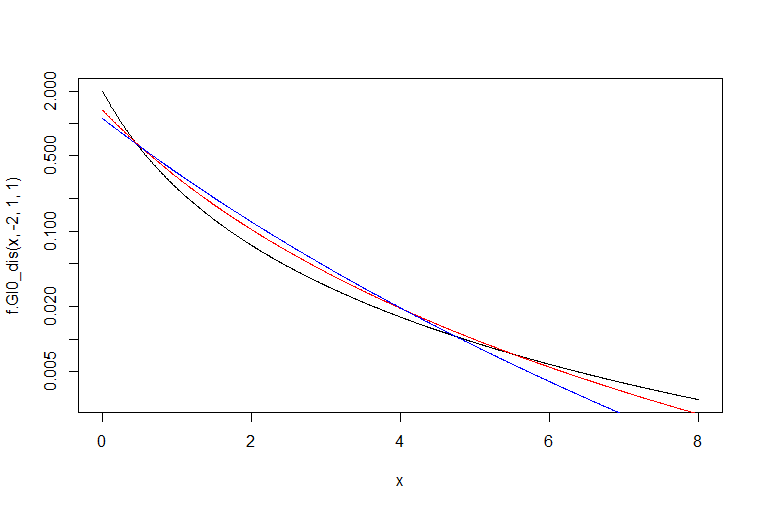
\includegraphics[width=.45\linewidth]{G_alpha_semilog.png}}\ 
	\caption{Densities in linear and semilogarithmic scale of $\mathcal{G}^0$ distribution with unitary mean and L=1. Black, red, blue for $\alpha\in\{-2,-4,-10\}$, respectively.}
	\label{Fig:G_dis_alpha}
\end{figure*}

\begin{figure*}[htb]
	\centering
	\subfloat[$\alpha=-2,\gamma=1$ Densities \label{Fig:G_L}]{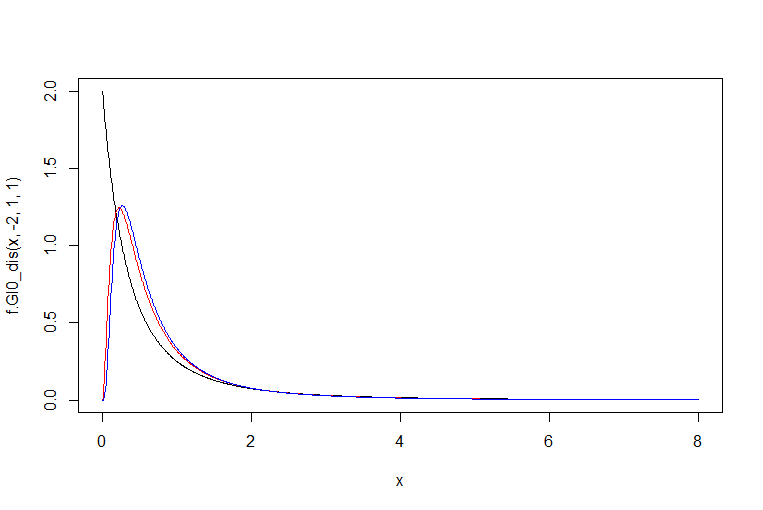
\includegraphics[width=.45\linewidth]{G_L.png}}\ 
	\subfloat[$\alpha=-2,\gamma=1$ Densities in semilog scale \label{Fig:G_L_semilog}]{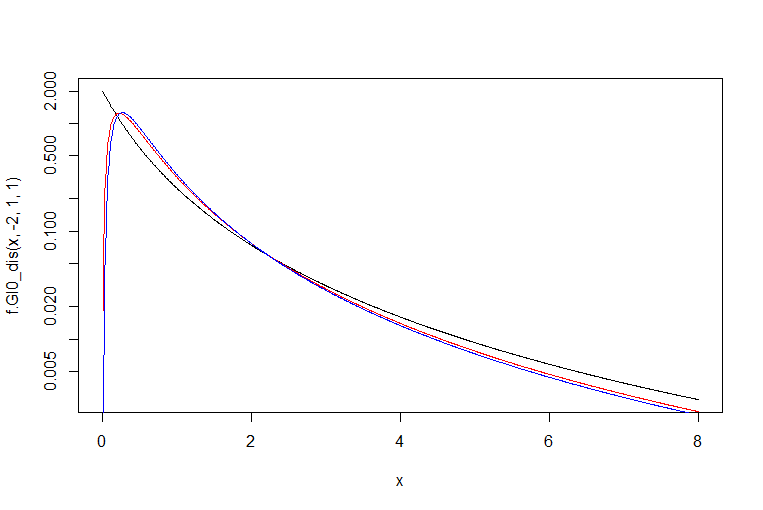
\includegraphics[width=.45\linewidth]{G_L_semilog.png}}\ 
	\caption{Densities in linear and semilogarithmic scale of $\mathcal{G}^0$ distribution with unitary mean and $\alpha=-2,\gamma=1$. Black, red, blue for $L\in\{1,3,5\}$, respectively.}
	\label{Fig:G_dis_L}
\end{figure*}

\section{Assignment 4 (2019-07-18/19)}
\subsection{Parameter estimation: Inference by analogy} 

For the Uniform distribution, the k-order moment estimator of $\theta$ is :
\begin{equation}
\widehat{\theta}_k = \sqrt[k]{\frac{k+1}{n} \sum_{i=1}^{n} U_i^k}
\end{equation}
Here, we can obtain three estimators of $\theta$ formed with $E(x), E(x^2), E(x^3)$:
\begin{equation}
\begin{split}
\widehat{\theta}_1 &= 2n^{-1}\sum_{i=1}^n U_i \\
\widehat{\theta}_2 &= \sqrt{3n^{-1}\sum_{i=1}^{n} U_i^2} \\
\widehat{\theta}_3 &= \sqrt[3]{4n^{-1} \sum_{i=1}^{n} U_i^3} \\
\end{split}
\end{equation}

 
For the (SAR) Gamma distribution characterized by the density:
\begin{equation}
f_\Gamma(z;L,\mu) = \frac{L^L}{\mu^{L}\Gamma(L)} z^{L-1} 
\exp\big\{ -L z / \mu
\big\}.
\label{eq:SARGammaDensity}
\end{equation}
We need two linearly independent equations to estimate $\bm{\theta}=(L,\mu)$. Knowing $E(Z)=\mu$ and $\operatorname{Var}(Z)=\mu^2/L$, we obtain the estimator of $\bm{\theta}$:
\begin{equation}
\begin{split}
\widehat{\mu} &= n^{-1}\sum_{i=1}^n Z_i \\
\widehat L &= \widehat{\mu}^2 / (n^{-1}\sum_{i=1}^n (Z_i - \widehat{\mu})^2) \\
\end{split}
\end{equation} 

Listing \ref{code:analogy} shows the estimators for the Uniform and the (SAR) Gamma distribution infered by analogy. For the Uniform distribution $\mathcal U_{(0,\pi)}$, we obtain the estimators $\widehat{\theta}_1=3.143274, \widehat{\theta}_2=3.142731, \widehat{\theta}_3=3.142359$. For the (SAR) Gamma distribution $\Gamma(2,7)$, we obtain the estimator $\widehat{\mu}=7.10646, \widehat L=1.961167$.

\begin{lstlisting}[caption={Parameter estimation for the Uniform and the (SAR) Gamma distribution (Inference by analogy)},label={code:analogy}]
## Uniform distribution  U(0,theta)
> x <- runif(1000000,min=0,max=pi)
>
> # Inference from E(x)
> (theta.hat.Mom1 <- 2*mean(x))
[1] 3.143274
> # Inference from E(x^2)
> (theta.hat.Mom2 <- sqrt(3*mean(x^2)))
[1] 3.142731
> # Inference from E(x^3)
> (theta.hat.Mom3 <- (4*mean(x^3))^(1/3))
[1] 3.142359

## Gamma distribution Gamma(mu,L) --- rgamma(n,L,L/mu)
> x <- rgamma(1000,2,2/7)
>
> (mu.hat <- mean(x))
[1] 7.10646
> (L.hat <- mu.hat^2 /var(x))
[1] 1.961167
\end{lstlisting}


\subsection{Fit the histogram with Exponential and $\mathcal{G}^0$ distribution.}

In this part, I will first give some conclusions about parameter estimation for the Exponential and $\mathcal{G}^0$ distribution. Then I will analyze a real data from an urban area.

For the Exponential distribution characterized by the density:
\begin{equation}
f_Z(z;\theta) = \theta^{-1} e^{-z/\theta}
\end{equation}
The $k$-order moment of $Z$ is given by:
\begin{equation}
\operatorname{E}Z^k = k!\theta^k
\label{eq:MomExp}
\end{equation}

\begin{itemize}
	\item Inference by analogy

	Based on $\operatorname{E}(Z)= \theta$, we obtain the estimator $\breve{\theta}$:
	\begin{equation}
	\breve{\theta}= N^{-1}\sum_{n=1}^N Z_n
	\end{equation}

	
	\item Inference by maximum likelihood
	
	The maximum likelihood estimator of $\hat{\theta}$ is the maximum point of the reduced log-likelihood:
	\begin{equation}
	\ell(\theta;\bm Z) = -Nln(\theta)-\frac{1}{\theta}\sum_{n=1}^N Z_n
	\label{Eq:ReducedLogLikExp}
	\end{equation}
	When the derivative of $\ell(\theta;\bm Z)$ equals to zero, we obtain the ML estimator $\hat{\theta}=N^{-1}\sum_{n=1}^N Z_n$. Note that $\hat{\theta}=\breve{\theta}$.
\end{itemize}

For the $\mathcal{G}^0$ distribution characterized by the density:
\begin{equation}
f_Z(z;\alpha,\gamma,L) = \frac{L^L \Gamma(L-\alpha)}{\gamma^\alpha \Gamma(L) \Gamma(\alpha)}
\frac{z^L}{(\gamma+Lz)^\alpha}
\end{equation}
The $k$-order moment of $Z$ is given by:
\begin{equation}
\operatorname{E}Z^k = \Big(\frac{\gamma}{L}\Big)^k
\frac{\Gamma(-\alpha-k)}{\Gamma(-\alpha)}
\frac{\Gamma(L+k)}{\Gamma(L)}
\label{eq:MomGI0}
\end{equation}
\begin{itemize}
	\item Inference by analogy
	
	Based on $\operatorname{E}(Z)= \frac{\gamma}{-\alpha-1}$ and $\operatorname{E}(Z^2)= \frac{\gamma^2}{L}\frac{L+1}{(-\alpha-1)(-\alpha-2)}$, we obtain the estimators $\breve{\alpha}, \breve{\gamma}$:
	\begin{equation}
	\begin{split}
	\breve{\alpha}	& = -2-\frac{L+1}{L\, m_2/m_1^2}\\
	\breve{\gamma}	& = m_1 \Big(2+\frac{L+1}{L\, m_2/m_1^2}\Big) \\
	\end{split}
	\end{equation}
	where $m_1, m_2$ are the first and second sample moments.
	
	\item Inference by maximum likelihood
	
	The maximum likelihood estimator of $\hat{\alpha}, \hat{\gamma}$ is the maximum point of the reduced log-likelihood:
	\begin{equation}
	\ell(\alpha,\gamma;\widehat L, \bm Z) = 
	\frac{\Gamma(\widehat L-\alpha)}{\gamma^\alpha \Gamma(-\alpha)} +
	\widehat L \sum_{n=1}^N \log\frac{Z_n}{\gamma+\widehat L Z_n} + 
	\alpha \sum_{n=1}^N \log(\gamma + \widehat L Z_n)
	\label{Eq:ReducedLogLikGI0}
	\end{equation}
\end{itemize}


Here we will analyze \textit{UrbanHV} data, shown in Fig.\ref{Fig:Urban}\subref{Fig:Urban_HV}. Fig.\ref{Fig:Urban}\subref{Fig:Urban_HV_hist}\subref{Fig:Urban_HV_hist_res} show the histogram and the restricted histogram of the data. 

The codes in Listing \ref{code:exp_estim}, \ref{code:G_mom_estim}, \ref{code:G_ML_estim} implement the estimator of Exponential distribution, the moment estimator of $\mathcal{G}^0$ distribution and the ML estimator of $\mathcal{G}^0$ distribution, respectively. Here we assume L = 1 for $\mathcal{G}^0$ distribution. For exponential distribution, we obtain $\hat{\theta}=45337.62$, and for $\mathcal{G}^0$ distribution, we obtain $\breve{\alpha}=-2.20801, \breve{\gamma}=100105.9$ estimated by the moments, $\hat{\alpha}=-2.662928, \hat{\gamma}=62808.457105$ estimated by the maximum likelihood. Fig.\ref{Fig:Fit_UrbanHV} shows the restricted histogram and fitted exponential densities (black) and $\mathcal{G}^0$ densities with the parameters estimated by the moments (blue) and maximum likelihood (red). According to Fig.\ref{Fig:Fit_UrbanHV}, $\mathcal{G}^0$ distribution with parameters estimated by maximum likelihood fit this data better.


\begin{figure}[htbp]
	\centering
	\subfloat[Image \label{Fig:Urban_HV}]{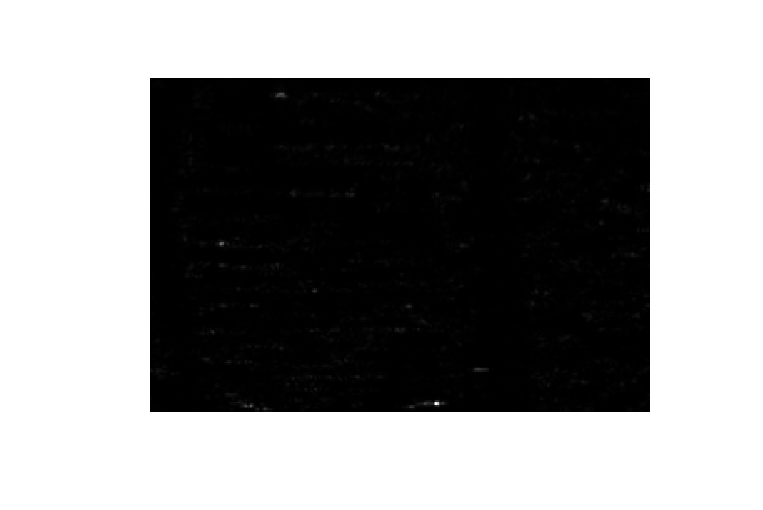
\includegraphics[width=.3\linewidth]{Urban_HV.png}}\ 
	\subfloat[Histogram \label{Fig:Urban_HV_hist}]{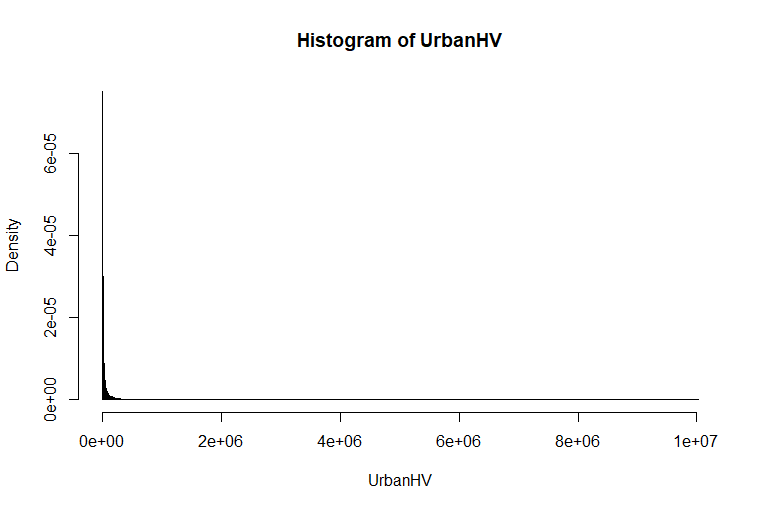
\includegraphics[width=.3\linewidth]{Urban_HV_hist.png}}\ 
	\subfloat[Restricted histogram \label{Fig:Urban_HV_hist_res}]{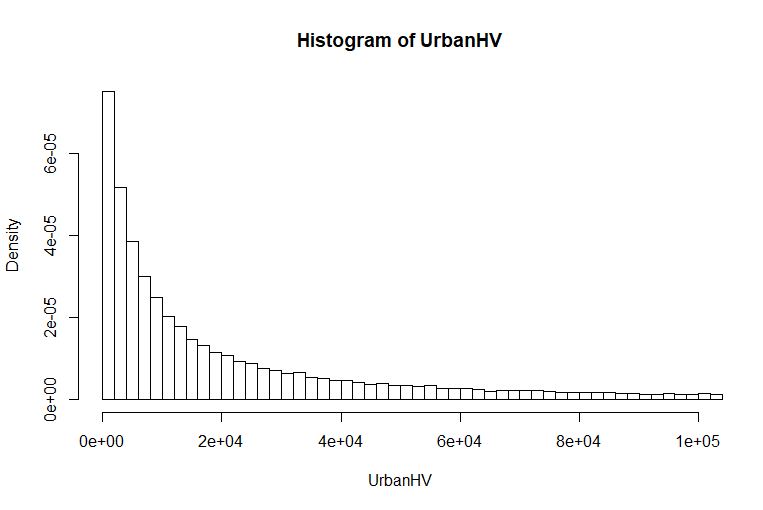
\includegraphics[width=.3\linewidth]{Urban_HV_hist_res.png}}\ 
	\caption{Image and histograms of data \textit{UrbanHV}}
	\label{Fig:Urban}
\end{figure}

\begin{lstlisting}[caption={Plot the data},label={code:plot_hist}]
## Plot data
plot(imagematrix(normalize(UrbanHV)))
hist(UrbanHV,probability = TRUE, breaks = "FD")
hist(UrbanHV,probability = TRUE, breaks = "FD",xlim = c(0,100000))
x <- seq(0,100000,length.out = 100000)
\end{lstlisting}

\begin{lstlisting}[caption={The estimator of Exponential distribution},label={code:exp_estim}]
## estimator of Exponential distribution
E.Est.m1 <- function(z)
{
mean(z)
}
E.estim.Mom <- E.Est.m1(UrbanHV)
E.Mom.fit <- dexp(x,rate=1/E.estim.Mom)
\end{lstlisting}

\begin{lstlisting}[caption={The moment estimator of $\mathcal{G}^0$ distribution},label={code:G_mom_estim}]
## Moment estimator of GI0 distribution
G.Est.m1m2 <- function(z,L)
{
m1<-mean(z)
m2<-mean(z^2)
m2m12 <- m2/m1^2
a <- -2-(L+1)/(L*m2m12)
g <- m1*(2+(L+1)/(L*m2m12))
return(list("alpha"=a,"gamma"=g))
}
G.estim.Mom <- G.Est.m1m2(UrbanHV,1)
G.Mom.fit <- f.GI0_dis(x,G.estim.Mom$alpha,G.estim.Mom$gamma,1)
\end{lstlisting}

\begin{lstlisting}[caption={The ML estimator of $\mathcal{G}^0$ distribution},label={code:G_ML_estim}]
# Loglikelihood of GI0(alpha,gamma,1)
G.LogLikelihood_L1 <- function(params)
{
p_alpha <- -abs(params[1])
p_gamma <- abs(params[2])
p_L <- abs(params[3])
n <- length(z)
return (n*(lgamma(p_L-p_alpha)-p_alpha*log(p_gamma)-lgamma(-p_alpha))+(p_alpha-p_L)*sum(log(p_gamma+z*p_L)))
}
z <- UrbanHV
G.estim.ML <- maxNR(G.LogLikelihood_L1,start=c(G.estim.Mom$alpha,G.estim.Mom$gamma,1),activePar=c(TRUE,TRUE,FALSE))$estimate[1:2]
G.ML.fit <- f.GI0_dis(x,G.estim.ML[1],G.estim.ML[2],1)
\end{lstlisting}

\begin{figure}[htbp]
	\centering
	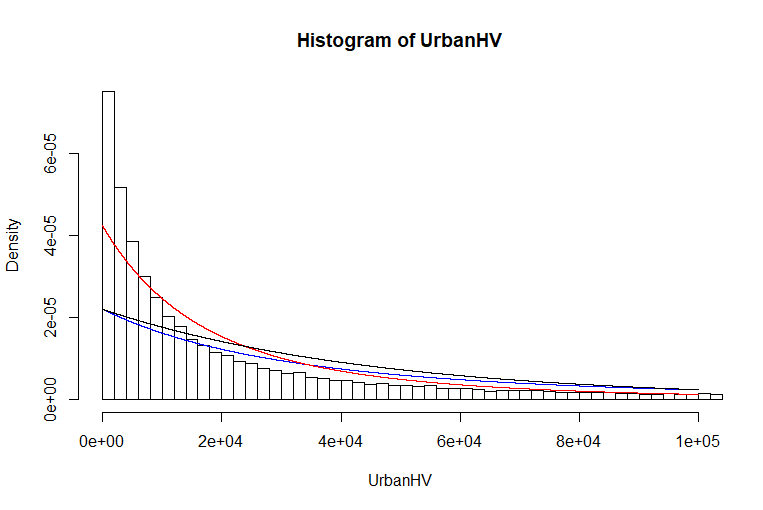
\includegraphics[width=.9\linewidth]{Fit_UrbanHV.png}
	\caption{Restricted histogram and fitted exponential densities (black) and $\mathcal{G}^0$ densities with the parameters estimated by the moments (blue) and maximum likelihood (red) methods.}
	\label{Fig:Fit_UrbanHV}
\end{figure}


\subsection{Compare estimators with a Monte Carlo experiment.}
Consider the Exponential distribution, we can obtain three estimators:
\begin{itemize}
	\item The maximum likelihood and first moment estimator $\widehat\mu$: 
	\begin{equation}
	\widehat{\mu} = \frac{1}{n}\sum_{i=1}^n Z_i
	\end{equation}
	\item The median estimator $\breve{\mu}$:
	\begin{equation}
	\breve{\mu} = \frac{1}{\ln 2} q_{1/2} (z_1,\dots,z_n)
	\end{equation}
	\item The bootstrapped median estimator $\widetilde{\mu}$.
\end{itemize}


The codes in Listing \ref{code:monte carlo} implement a Monte Carlo experiment. In the experiment, I set $\mu=1$, $R=300$, the sample size $n\in\{3,5,10,20,30,40,50,60,70,80,90,100,500,1000,10000\}$, and the number of replications $r=2\times 10^6/n$. For each $(n,\mu)$ we can obtain the bias, and the mean quadratic error of $\widehat{\mu}$, $\breve{\mu}$ and $\widetilde{\mu}$. Fig.\ref{Fig:Monte_Carlo} shows how the bias(\ref{Fig:Monte_Carlo}\subref{Fig:M_bias}) and the mean square error(\ref{Fig:Monte_Carlo}\subref{Fig:M_mse}) change with the number of samples $n$.

From Fig.\ref{Fig:Monte_Carlo}\subref{Fig:M_bias} we can see that when sample size is large enough, the biases of $\widehat{\mu}$, $\breve{\mu}$ and $\widetilde{\mu}$ are close, which means we can choose any one of these three estimators. However, when sample size is small, the bias of $\breve{\mu}$ is large while the bias of $\widehat{\mu}$, $\widetilde{\mu}$ are both small (when sample size $n>5$). When $n=3$, though $\widetilde{\mu}$ is much smaller than $\breve{\mu}$, it is still larger than $\widehat{\mu}$. The bias of $\widehat{\mu}$ is always small for almost every sample size.

From Fig.\ref{Fig:Monte_Carlo}\subref{Fig:M_mse} we can see that when sample size is large enough, the MSE of $\widehat{\mu}$, $\breve{\mu}$ and $\widetilde{\mu}$ are close too. While when sample size is small, the MSE of  $\breve{\mu}$ is smaller than $\widetilde{\mu}$ and larger than $\widehat{\mu}$. The MSEs of all these estimators show a trend of decreasing with the increase of sample size $n$.

Considering both bias and MSE, maximum likelihood estimator has the best performance.


\begin{lstlisting}[caption={Monte Carlo experiment for comparing estimators of Exponential distribution},label={code:monte carlo}]
library(gtools)
require(gtools)
set.seed(123)
## bootstrapped median estimator
E.est.median.bootstrap <- function(z,R){
theta.hat <- median(z)/log(2)
sample_size <- length(z)

if(R>(sample_size^sample_size)){
m.Bootstrap <- permutations(sample_size,sample_size,z,set=TRUE, repeats.allowed=TRUE)
return(2*theta.hat - mean(unlist(lapply(m.Bootstrap,median)))/log(2))
}
else{
v.Bootstrap <- rep(0,R)
for(idx in 1:R){
x <- sample(z,replace = TRUE)
v.Bootstrap[idx] <- median(x)/log(2)
}
}
return (2*theta.hat-mean(v.Bootstrap))
}

## N for sample size
N<-c(3,5,10,20,30,40,50,60,70,80,90,100,500,1000,10000)
BiasMSE <- matrix(nrow=15,ncol=7)

i<-0
for(n in N){
i<-i+1
r<- ceiling(2*10^6/n)
v.mu.ML <- array(rep(0,r))
v.mu.Med <- array(rep(0,r))
v.mu.BootMed <- array(rep(0,r))
for (j in 1:r)
{
z<- rexp(n)
# First moment estimator or ML estimator
v.mu.ML[j]<- mean(z)
# Median estimator
v.mu.Med[j]<- median(z)/log(2)
# Bootstrapped median estimator
v.mu.BootMed[j]<- E.est.median.bootstrap(z,300)
}

bias.ML<- mean(v.mu.ML)-1
mse.ML <- mean((v.mu.ML-1)^2)
bias.Med<- mean(v.mu.Med)-1
mse.Med <- mean((v.mu.Med-1)^2)
bias.BootMed<- mean(v.mu.BootMed)-1
mse.BootMed <- mean((v.mu.BootMed-1)^2)

BiasMSE[i,]<-c(N[i],bias.ML,mse.ML,bias.Med,mse.Med,bias.BootMed,mse.BootMed)
}

# abs(Bias)
plot(BiasMSE[,1],abs(BiasMSE[,2]),type="l",col="red",log = "x",ylim=c(0,0.3),lwd=2)
lines(BiasMSE[,1],abs(BiasMSE[,4]),col="black",lwd=2)
lines(BiasMSE[,1],abs(BiasMSE[,6]),col="blue",lwd=2)
# MSE
plot(BiasMSE[,1],BiasMSE[,3],type="l",col="red",log = "x",ylim=c(0,1.5),lwd=2)
lines(BiasMSE[,1],BiasMSE[,5],col="black",lwd=2)
lines(BiasMSE[,1],BiasMSE[,7],col="blue",lwd=2)
}
\end{lstlisting}

\begin{figure}[htbp]
	\centering
	\subfloat[The bias \label{Fig:M_bias}]{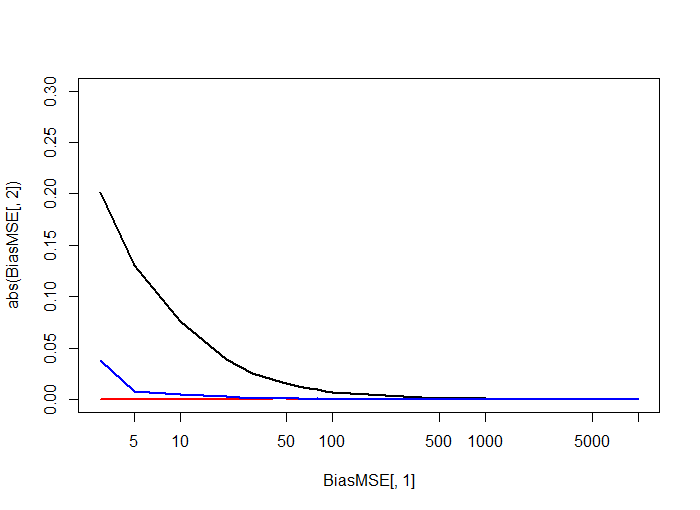
\includegraphics[width=.4\linewidth]{M_bias.png}}\ 
	\subfloat[The mean square error \label{Fig:M_mse}]{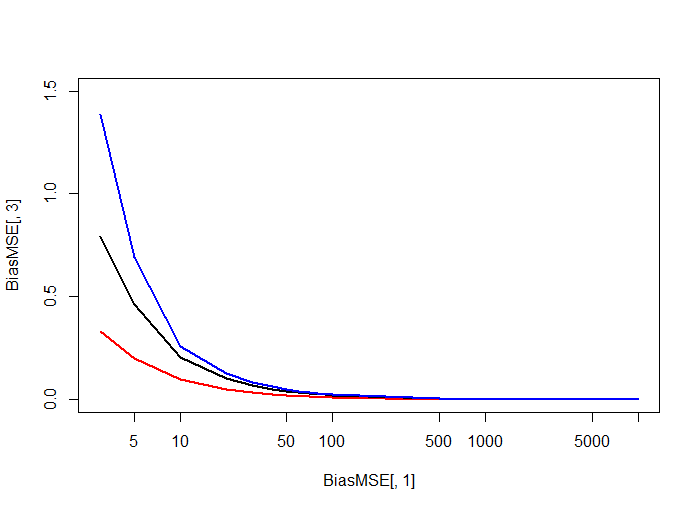
\includegraphics[width=.4\linewidth]{M_mse.png}}\ 
	\caption{The dependence of the bias and the mean square error on the sample size $n$.}
	\label{Fig:Monte_Carlo}
\end{figure}

\end{document}



